% Stan Warford
% Pepperdine University
% File: 221-Equations.tex
% The equation handout for Gries & Schneider, A Logical Approach to Discrete Math
% with modifications

\documentclass{amsart}

\usepackage{fontspec}
\usepackage[slantedGreek]{mathptmx}
\usepackage{amssymb,latexsym,graphics}
\usepackage{verbatim}

% For Dr. Warford's computer
\begin{comment}
\setmainfont{Times}[ItalicFont    ={* Italic},
                    BoldFont      ={* Bold},
                    BoldItalicFont={* Bold Italic}]
\setsansfont{Helvetica}
\end{comment}

% For Alex's computer
%\begin{comment}
\setmainfont{Times New Roman}[ItalicFont    ={* Italic},
                    BoldFont      ={* Bold},
                    BoldItalicFont={* Bold Italic}]
\setsansfont{Arial}
%\end{comment}

\newcommand{\lgap}{2pt}                             % Line gap
\newcommand{\llgap}{6pt}                            % Larger line gap
\newcommand{\lllgap}{12pt}                          % Larger yet line gap
\newcommand{\equivs}{\ensuremath{\;\equiv\;}}       % Equivales with space
\newcommand{\equivss}{\ensuremath{\;\;\equiv\;\;}}  % Equivales with double space
\newcommand{\nequiv}{\ensuremath{\not\equiv}}       % Inequivalent
\newcommand{\impl}{\ensuremath{\Rightarrow}}        % Implies
\newcommand{\impls}{\ensuremath{\;\Rightarrow\;}}   % Implies with space
\newcommand{\nimpl}{\ensuremath{\not\Rightarrow}}   % Does not imply
\newcommand{\foll}{\ensuremath{\Leftarrow}}         % Follows from
\newcommand{\nfoll}{\ensuremath{\not\Leftarrow}}    % Does not follow from
\newcommand{\mymod}{\;\textbf{mod}\;}
\newcommand{\mygcd}{\;\textbf{gcd}\;}
\newcommand{\mylcm}{\;\textbf{lcm}\;}


% These macros are used for quantifications. Thanks to David Gries for sharing
\newcommand{\thedr}{\rule[-.25ex]{.32mm}{1.75ex}}   % Symbol that separates dummy from range in quantification
\newcommand{\dr}{\;\,\thedr\,\;}                    % Symbol that separates dummy from range, with spacing
\newcommand{\rb}{:}                                 % Symbol that separates range from body in quantification
\newcommand{\drrb}{\;\thedr\,{:}\;}                 % Symbol that separates dummy from body when range is missing
\newcommand{\all}{\forall}                          % Universal quantification
\newcommand{\ext}{\exists}                          % Existential quantification
\newcommand{\guard}{[\negthinspace ]}               % Rectangle for guard

% Macros for proof hints
\newcommand{\Gll} {\langle}                         % Open hint
\newcommand{\Ggg} {\rangle}                         % Close hint
\newlength{\Glllength}                              % Length of open hint symbol
\settowidth{\Glllength}{$.\Gll$}
\newcommand{\Hint}[1]     {\ \ \ $\Gll              \mbox{#1} \Ggg$ }   % Single line hint
\newcommand{\Hintfirst}[1]{\ \ \ $\Gll              \mbox{#1}$ }        % First line of multiline hint
\newcommand{\Hintmid}[1]  {\ \ $\hspace{\Glllength} \mbox{#1}$ }        % Middle line of multiline hint
\newcommand{\Hintlast}[1] {\ \ $\hspace{\Glllength} \mbox{#1} \Ggg$ }   % Last line of multiline hint

% Single and double quotes
\newcommand{\Lq}{\mbox{`}}
\newcommand{\Rq}{\mbox{'}}
\newcommand{\Lqq}{\mbox{``}}
\newcommand{\Rqq}{\mbox{''}}

\begin{document}
\title[Theorems from LADM]{Theorems from Gries and Schneider's LADM}
\author{J.~Stanley Warford}
\address{Natural Science Division\\
         Pepperdine University\\
         Malibu, CA 90265}
\email{Stan.Warford@pepperdine.edu}
\urladdr{http://mccarthy.cslab.pepperdine.edu/\~{}warford/}
\date{\today}
\begin{abstract}
This is a collection of the axioms and theorems in Gries and Schneider's
book \textit{A Logical Approach to Discrete Math} (LADM), Springer-Verlag, 1993.
The numbering is consistent with that text.
Additional theorems not included or numbered in LADM are indicated by a three-part
number.
This document serves as a reference for homework exercises and taking exams.
\end{abstract}

\maketitle

\section*{Table of Precedences}
\begin{tabbing}
(m)\;\=\kill
(a)\>$[x := e]$ (textual substitution) \qquad \hfill (highest precedence)\\
(b)\>. (function application)\\
(c)\>unary prefix operators: $+$\quad $-$\quad $\neg$\quad $\#$\quad $\thicksim$\quad $\mathcal{P}$\\
(d)\>$**$\\
(e)\>$\cdot$\quad $/$\quad $\div$\quad \textbf{mod}\quad \textbf{gcd}\\
(f)\>$+$\quad $-$\quad $\cup$\quad $\cap$\quad $\times$\quad $\circ$\quad $\bullet$\\
(g)\>$\downarrow$\quad $\uparrow$\\
(h)\>$\#$\\
(i)\>$\triangleleft$\quad $\triangleright$\quad \textasciicircum\\
(j)\>$=$\quad $<$\quad $>$\quad $\in$\quad $\subset$\quad $\subseteq$\quad $\supset$\quad $\supseteq$\quad $\mid$
\qquad (conjunctional, see page 29)\\
(k)\>$\lor$\quad $\land$\\
(l)\>$\impl$\quad $\foll$\\
(m)\>$\equiv$\\
\end{tabbing}
\par
All nonassociative binary infix operators associate from left to right except $**$, $\triangleleft$, and $\impl$,
which associate from right to left.

The operators on lines (j), (l), and (m) may have a slash $/$ through them to denote negation---e.g.
$b\nequiv c$ is an abbreviation for $\neg(b \equiv c)$.

\section*{Some Basic Types}
\begin{tabbing}
$positive reals$\quad\quad\= Symbol\quad\quad\=\kill
Name                \>Symbol           \> Type (set of values)\\[-8pt]
\rule{5in}{0.5pt}\\
$integer$           \>$\mathbb{Z}$     \> integers: $\ldots , -3, -2, -1, 0, 1, 2, 3, \ldots$\\[\lgap]
$nat$               \>$\mathbb{N}$     \> natural numbers: $0, 1, 2, \ldots$\\[\lgap]
$positive$          \>$\mathbb{Z}^{+}$ \> positive integers: $1, 2, 3, \ldots$\\[\lgap]
$negative$          \>$\mathbb{Z}^{-}$ \> negative integers: $-1, -2, -3, \ldots$\\[\lgap]
$rational$          \>$\mathbb{Q}$     \> rational numbers: $i/j$ for $i,j$ integers, $j\ne 0$\\[\lgap]
$reals$             \>$\mathbb{R}$     \> real numbers\\[\lgap]
$positive$ $reals$  \>$\mathbb{R}^{+}$ \> positive real numbers\\[\lgap]
$bool$              \>$\mathbb{B}$     \> booleans: $true, false$
\end{tabbing}

\section*{Theorems of the Propositional Calculus}

\subsection*{Equivalence and $true$}
\begin{tabbing}
(99.99.9)\;\=\kill
(3.1)\>\textbf{Axiom, Associativity of $\equiv$ :}\quad $((p\equiv q) \equiv r)\equivs (p\equiv (q\equiv r))$\\[\lgap]
(3.2)\>\textbf{Axiom, Symmetry of $\equiv$ :}\quad $p\equiv q \equiv q\equiv p$\\[\lgap]
(3.3)\>\textbf{Axiom, Identity of $\equiv$ :}\quad $true\equiv q \equiv q$\\[\lgap]
(3.4)\>$true$\\[\lgap]
(3.5)\>\textbf{Reflexivity of $\equiv$ :}\quad $p\equiv p$\\
\end{tabbing}

\subsection*{Negation, inequivalence, and $false$}
\begin{tabbing}
(99.99.9)\;\=\kill
(3.8)\>\textbf{Axiom, Definition of $false$ :}\quad $false\equiv \neg true$\\[\lgap]
(3.9)\>\textbf{Axiom, Distributivity of $\neg$ over $\equiv$ :}\quad $\neg (p\equiv q) \equivs \neg p \equiv q$\\[\lgap]
(3.10)\>\textbf{Axiom, Definition of $\nequiv$ :}\quad $(p\nequiv q)\equivs\neg(p\equiv q)$\\[\lgap]
(3.11)\>$\neg p \equiv q \equiv p \equiv \neg q$\\[\lgap]
(3.12)\>\textbf{Double negation:}\quad $\neg\neg p\equiv p$\\[\lgap]
(3.13)\>\textbf{Negation of $false$:}\quad $\neg false\equiv true$\\[\lgap]
(3.14)\>$(p\nequiv q)\equivs\neg p\equiv q$\\[\lgap]
(3.15)\>$\neg p\equiv p\equiv false$\\[\lgap]
(3.16)\>\textbf{Symmetry of $\nequiv$ :}\quad $(p\nequiv q) \equivs (q\nequiv p)$\\[\lgap]
(3.17)\>\textbf{Associativity of $\nequiv$ :}\quad $((p\nequiv q) \nequiv r)\equivs (p\nequiv (q\nequiv r))$\\[\lgap]
(3.18)\>\textbf{Mutual associativity:}\quad $((p\nequiv q) \equiv r)\equivs (p\nequiv (q\equiv r))$\\[\lgap]
(3.19)\>\textbf{Mutual interchangeability:}\quad $p\nequiv q \equiv r\equivss p\equiv q\nequiv r$\\
(3.19.1)\>$p\nequiv p \nequiv q\equivs q$\\
\end{tabbing}

\subsection*{Disjunction}
\begin{tabbing}
(99.99.9)\;\=\kill
(3.24)\>\textbf{Axiom, Symmetry of $\lor$ :}\quad $p\lor q \equiv q\lor p$\\[\lgap]
(3.25)\>\textbf{Axiom, Associativity of $\lor$ :}\quad $(p\lor q) \lor r\equiv p\lor (q\lor r)$\\[\lgap]
(3.26)\>\textbf{Axiom, Idempotency of $\lor$ :}\quad $p\lor p \equiv p$\\[\lgap]
(3.27)\>\textbf{Axiom, Distributivity of $\lor$ over $\equiv$ :}\quad $p\lor (q\equiv r)\equiv p\lor q\equiv p\lor r$\\[\lgap]
(3.28)\>\textbf{Axiom, Excluded middle:}\quad $p\lor\neg p$\\[\lgap]
(3.29)\>\textbf{Zero of $\lor$ :}\quad $p\lor true\equiv true$\\[\lgap]
(3.30)\>\textbf{Identity of $\lor$ :}\quad $p\lor false\equiv p$\\[\lgap]
(3.31)\>\textbf{Distributivity of $\lor$ over $\lor$ :}\quad $p\lor (q\lor r)\equiv (p\lor q)\lor (p\lor r)$\\[\lgap]
(3.32)\>$p\lor q\equiv p\lor\neg q\equiv p$\\
\end{tabbing}

%\newpage

\subsection*{Conjunction}
\begin{tabbing}
(99.99.9)\;\=(m)\;\=\kill
(3.35)\>\textbf{Axiom, Golden rule:}\quad $p\land q\equivs p\equivs q\equivs p\lor q$\\[\lgap]
(3.36)\>\textbf{Symmetry of $\land$ :}\quad $p\land q \equiv q\land p$\\[\lgap]
(3.37)\>\textbf{Associativity of $\land$ :}\quad $(p\land q) \land r\equiv p\land (q\land r)$\\[\lgap]
(3.38)\>\textbf{Idempotency of $\land$ :}\quad  $p\land p \equiv p$\\[\lgap]
(3.39)\>\textbf{Identity of $\land$ :}\quad $p\land true\equiv p$\\[\lgap]
(3.40)\>\textbf{Zero of $\land$ :}\quad $p\land false\equiv false$\\[\lgap]
(3.41)\>\textbf{Distributivity of $\land$ over $\land$ :}\quad $p\land (q\land r)\equiv (p\land q)\land (p\land r)$\\[\lgap]
(3.42)\>\textbf{Contradiction:}\quad $p \land \neg p \equiv false$\\[\lgap]
(3.43)\>\textbf{Absorption:}\\
      \> (a)\> $p \land (p \lor q) \equiv p$\\[\lgap]
      \> (b)\> $p \lor (p \land q) \equiv p$\\[\lgap]
(3.44)\>\textbf{Absorption:}\\
      \> (a)\> $p \land (\neg p \lor q) \equiv p \land q$\\[\lgap]
      \> (b)\> $p \lor (\neg p \land q) \equiv p \lor q$\\[\lgap]
(3.45)\>\textbf{Distributivity of $\lor$ over $\land$ :}\quad $p\lor (q\land r)\equiv (p\lor q)\land (p\lor r)$\\[\lgap]
(3.46)\>\textbf{Distributivity of $\land$ over $\lor$ :}\quad $p\land (q\lor r)\equiv (p\land q)\lor (p\land r)$\\[\lgap]
(3.47)\>\textbf{De Morgan:}\\
      \> (a)\> $\neg (p \land q) \equiv \neg p \lor \neg q$\\[\lgap]
      \> (b)\> $\neg (p \lor q) \equiv \neg p \land \neg q$\\[\lgap]
(3.48)\>$p\land q\equivs p\equivs p\land \neg q\equivs \neg p$\\[\lgap]
(3.49)\>$p\land (q\equiv r)\equivs p\land q\equivs p\land r \equivs p$\\[\lgap]
(3.50)\>$p\land (q\equiv p)\equivs p\land q$\\[\lgap]
(3.51)\>\textbf{Replacement:}\quad $(p \equiv q) \land (r \equiv p) \equivss (p \equiv q) \land (r \equiv q)$\\[\lgap]
(3.52)\>\textbf{Definition of $\equiv$ :}\quad $p \equiv q \equivs (p \land q) \lor (\neg p \land \neg q)$\\[\lgap]
(3.53)\>\textbf{Exclusive or:}\quad $p \nequiv q \equivs (\neg p \land q) \lor (p \land \neg q)$\\[\lgap]
(3.55)\>$(p\land q)\land r \equivs p \equivs q \equivs r \equivs p\lor q \equivs q\lor r \equivs r\lor p \equivs p \lor q\lor r$\\
\end{tabbing}

%\newpage

\subsection*{Implication}
\begin{tabbing}
(99.99.9)\;\=(m)\;\=\kill
(3.57)\>\textbf{Axiom, Definition of Implication:}\quad $p\impl q \equivs p\lor q \equivs q$\\[\lgap]
(3.58)\>\textbf{Axiom, Consequence:}\quad $p\foll q \equivs q\impl p$\\[\lgap]
(3.59)\>\textbf{Definition of Implication:}\quad $p\impl q \equivs \neg p \lor q$\\[\lgap]
(3.60)\>\textbf{Definition of Implication:}\quad $p\impl q \equivs p\land q \equivs p$\\[\lgap]
(3.61)\>\textbf{Contrapositive:}\quad $p\impl q \equivs \neg q\impl \neg p$\\[\lgap]
(3.62)\>$p\impl (q\equiv r) \equivs p\land q\equivs p\land r$\\[\lgap]
(3.63)\>\textbf{Distributivity of $\impl$ over $\equiv$ :}\quad $p\impl (q\equiv r)\equivs (p\impl q)\equivs (p\impl r)$\\[\lgap]
(3.64)\>$p\impl (q\impl r) \equivs (p\impl q)\impl (p\impl r)$\\[\lgap]
(3.65)\>\textbf{Shunting:}\quad $p\land q\impl r\equivs p\impl (q\impl r)$\\[\lgap]
(3.66)\>$p\land (p\impl q) \equivs p\land q$\\[\lgap]
(3.67)\>$p\land (q\impl p) \equivs p$\\[\lgap]
(3.68)\>$p\lor (p\impl q) \equivs true$\\[\lgap]
(3.69)\>$p\lor (q\impl p) \equivs q\impl p$\\[\lgap]
(3.70)\>$p\lor q \impl p\land q \equivs p \equivs q$\\[\lgap]
(3.71)\>\textbf{Reflexivity of $\impl$ :}\quad $p\impl p \equivs true$\\[\lgap]
(3.72)\>\textbf{Right zero of $\impl$ :}\quad $p\impl true \equivs true$\\[\lgap]
(3.73)\>\textbf{Left identity of $\impl$ :}\quad $true\impl p \equivs p$\\[\lgap]
(3.74)\>$p\impl false \equivs \neg p$\\[\lgap]
(3.75)\>$false\impl p \equivs true$\\[\lgap]
\end{tabbing}
\newpage
\begin{tabbing}
(99.99.9)\;\=(m)\;\=\kill

(3.76)\>\textbf{Weakening/strengthening:}\\
      \> (a)\> $p\impl p\lor q$\quad \quad \quad (Weakening the consequent)\\[\lgap]
      \> (b)\> $p\land q \impl p$\quad \quad \quad (Strengthening the antecedent)\\[\lgap]
      \> (c)\> $p\land q \impl p\lor q$\quad \quad \quad (Weakening/strengthening)\\[\lgap]
      \> (d)\> $p\lor (q\land r) \impl p\lor q$\\[\lgap]
      \> (e)\> $p\land q \impl p\land (q \lor r)$\\[\lgap]
(3.77)\>\textbf{Modus ponens:}\quad $p\land (p\impl q)\impl q$\\[\lgap]
(3.78)\>$(p\impl r) \land (q\impl r) \equivs (p\lor q\impl r)$\\[\lgap]
(3.79)\>$(p\impl r) \land (\neg p\impl r) \equivs r$\\[\lgap]
(3.80)\>\textbf{Mutual implication:}\quad $(p\impl q) \land (q\impl p) \equivs (p\equiv q)$\\[\lgap]
(3.81)\>\textbf{Antisymmetry:}\quad $(p\impl q) \land (q\impl p) \impl (p\equiv q)$\\[\lgap]
(3.82)\>\textbf{Transitivity:}\\
      \> (a)\> $(p\impl q) \land (q\impl r) \impl (p\impl r)$\\[\lgap]
      \> (b)\> $(p\equiv q) \land (q\impl r) \impl (p\impl r)$\\[\lgap]
      \> (c)\> $(p\impl q) \land (q\equiv r) \impl (p\impl r)$\\[\lgap]
(3.82.1)\>\textbf{Transitivity of $\equiv$ :}\quad $(p\equiv q)\land (q\equiv r)\impl (p\equiv r)$\\
\end{tabbing}

\subsection*{Leibniz as an axiom}
\begin{tabbing}
(99.99.9)\;\=(m)\;\=\kill
This section uses the following notation: $E^{z}_{X}$ means $E[z := X]$.\\[\lgap]
(3.83)\>\textbf{Axiom, Leibniz:}\quad $e=f\impl E^{z}_{e} = E^{z}_{f}$\\[\lgap]
(3.84)\>\textbf{Substitution:}\\
      \> (a)\> $(e=f) \land E^{z}_{e} \equivs (e=f)\land E^{z}_{f}$\\[\lgap]
      \> (b)\> $(e=f) \impl E^{z}_{e} \equivs (e=f)\impl E^{z}_{f}$\\[\lgap]
      \> (c)\> $q\land (e=f) \impl E^{z}_{e} \equivs q\land (e=f)\impl E^{z}_{f}$\\[\lgap]
(3.85)\>\textbf{Replace by $true$:}\\
      \> (a)\> $p \impl E^{z}_{p} \equivs p\impl E^{z}_{true}$\\[\lgap]
      \> (b)\> $q\land p \impl E^{z}_{p} \equivs q\land p\impl E^{z}_{true}$\\[\lgap]
(3.86)\>\textbf{Replace by $false$:}\\
      \> (a)\> $E^{z}_{p} \impl p \equivs E^{z}_{false}\impl p$\\[\lgap]
      \> (b)\> $E^{z}_{p} \impl p\lor q \equivs E^{z}_{false}\impl p\lor q$\\[\lgap]
(3.87)\>\textbf{Replace by $true$:}\quad $p\land E^{z}_{p} \equivs p\land E^{z}_{true}$\\[\lgap]
(3.88)\>\textbf{Replace by $false$:}\quad $p\lor E^{z}_{p} \equivs p\lor E^{z}_{false}$\\[\lgap]
(3.89)\>\textbf{Shannon:}\quad $E^{z}_{p}\equivs (p\land E^{z}_{true}) \lor (\neg p\land E^{z}_{false})$\\
\end{tabbing}

\subsection*{Additional theorems concerning implication}
\begin{tabbing}
(99.99.9)\;\=(m)\;\=\kill
(4.1)\>$p\impl (q\impl p)$\\[\lgap]
(4.2)\>\textbf{Monotonicity of $\lor$ :}\quad $(p\impl q) \impl (p\lor r \impl q\lor r)$\\[\lgap]
(4.3)\>\textbf{Monotonicity of $\land$ :}\quad $(p\impl q) \impl (p\land r \impl q\land r)$\\[\lgap]
\end{tabbing}

\newpage

\subsection*{Proof techniques}
\begin{tabbing}
(99.99.9)\;\=(m)\;\=\kill
(4.4)\>\textbf{Deduction:}\quad To prove $P\impl Q$, assume $P$ and prove $Q$.\\[\lgap]
(4.5)\>\textbf{Case analysis:}\quad If $E^{z}_{true}$ and $E^{z}_{false}$ are theorems, then so is $E^{z}_{P}$.\\[\lgap]
(4.6)\>\textbf{Case analysis:}\quad $(p\lor q\lor r)\land (p\impl s)\land (q\impl s)\land (r\impl s)\impl s$\\[\lgap]
(4.7)\>\textbf{Mutual implication:}\quad To prove $P\equiv Q$, prove $P\impl Q$ and $Q\impl P$.\\[\lgap]
(4.9)\>\textbf{Proof by contradiction:}\quad To prove $P$, prove $\neg P\impl false$.\\[\lgap]
(4.12)\>\textbf{Proof by contrapositive:}\quad To prove $P\impl Q$, prove $\neg Q\impl \neg P$.\\
\end{tabbing}

\section*{General Laws of Quantification}
\begin{tabbing}
(99.99.9)\;\=(m)\;\=\kill
For symmetric and associative binary operator $\star$ with identity $u$.\\[\lgap]
(8.13)\>\textbf{Axiom, Empty range:}\quad $(\star x \dr false \rb P) =u$\\[\lgap]
(8.14)\>\textbf{Axiom, One-point rule:}\quad Provided $\neg occurs(\Lq x\Rq ,\Lq E\Rq)$,\\[\lgap]
      \>$(\star x\dr x=E\rb P) = P[x:=E]$\\[\lgap]
(8.15)\>\textbf{Axiom, Distributivity:}\quad Provided $P,Q:\mathbb{B}$ or $R$ is finite,\\[\lgap]
      \>$(\star x\dr R\rb P)\star (\star x\dr R\rb Q) = (\star x\dr R\rb P\star Q)$\\[\lgap]
(8.16)\>\textbf{Axiom, Range split:}\quad Provided $R\land S\equiv false$ and $P:\mathbb{B}$ or $R$ and $S$ are finite,\\[\lgap]
      \>$(\star x\dr R\lor S\rb P) = (\star x\dr R\rb P)\star (\star x\dr S\rb P)$\\[\lgap]
(8.17)\>\textbf{Axiom, Range split:}\quad Provided $P:\mathbb{B}$ or $R$ and $S$ are finite,\\[\lgap]
      \>$(\star x\dr R\lor S\rb P)\star (\star x\dr R\land S\rb P) = (\star x\dr R\rb P)\star (\star x\dr S\rb P)$\\[\lgap]
(8.18)\>\textbf{Axiom, Range split for idempotent $\star$ :}\quad Provided $P:\mathbb {B}$ or $R$ and $S$ are finite,\\[\lgap]
      \>$(\star x\dr R\lor S\rb P) = (\star x\dr R\rb P)\star (\star x\dr S\rb P)$\\[\lgap]
(8.19)\>\textbf{Axiom, Interchange of dummies:}\quad Provided $\star$ is idempotent or $R$ and $S$ are finite,\\[\lgap]
      \>$\neg occurs(\Lq y\Rq ,\Lq R\Rq)$, $\neg occurs(\Lq x\Rq ,\Lq Q\Rq)$,\\[\lgap]
      \>$(\star x\dr R\rb (\star y\dr Q\rb P)) = (\star y\dr Q\rb (\star x\dr R\rb P))$\\[\lgap]
(8.20)\>\textbf{Axiom, nesting:}\quad Provided $\neg occurs(\Lq y\Rq ,\Lq R\Rq)$,\\[\lgap]
      \>$(\star x,y\dr R\land Q\rb P) = (\star x\dr R\rb (\star y\dr Q\rb P))$\\[\lgap]
(8.21)\>\textbf{Axiom, Dummy renaming:}\quad Provided $\neg occurs(\Lq y\Rq ,\Lq R, P\Rq)$,\\[\lgap]
      \>$(\star x\dr R\rb P) = (\star y\dr R[x:=y]\rb P[x:=y])$\\[\lgap]
(8.22)\>\textbf{Change of dummy:}\quad Provided $\neg occurs(\Lq y\Rq ,\Lq R, P\Rq)$, and $f$ has an inverse,\\[\lgap]
      \>$(\star x\dr R\rb P) = (\star y\dr R[x:=f.y]\rb P[x:=f.y])$\\[\lgap]
(8.23)\>\textbf{Split off term:}\quad For $n$: $\mathbb{N}$,\\[\lgap]
      \> (a)\> $(\star i\dr 0\le i < n+1\rb P) = (\star i\dr 0\le i < n\rb P)\star P[i:=n]$\\[\lgap]
      \> (b)\> $(\star i\dr 0\le i < n+1\rb P) = P[i:=0]\star (\star i\dr 0< i < n+1\rb P)$\\[\lgap]
\end{tabbing}

\newpage

\section*{Theorems of the Predicate Calculus}

\subsection*{Universal quantification}
\begin{tabbing}
(99.99.9)\;\=(m)\;\=\kill
Notation: $(\star x\drrb P)$ means $(\star x\dr true\rb P)$.\\[\lgap]
(9.2)\>\textbf{Axiom, Trading:}\quad $(\all x\dr R\rb P)\equiv (\all x\drrb R\impl P)$\\[\lgap]
(9.3)\>\textbf{Trading:}\\[\lgap]
      \> (a)\> $(\all x\dr R\rb P)\equiv (\all x\drrb \neg R\lor P)$\\[\lgap]
      \> (b)\> $(\all x\dr R\rb P)\equiv (\all x\drrb R\land P\equiv R)$\\[\lgap]
      \> (c)\> $(\all x\dr R\rb P)\equiv (\all x\drrb R\lor P\equiv P)$\\[\lgap]
(9.4)\>\textbf{Trading:}\\[\lgap]
      \> (a)\> $(\all x\dr Q\land R\rb P)\equiv (\all x\dr Q\rb R\impl P)$\\[\lgap]
      \> (b)\> $(\all x\dr Q\land R\rb P)\equiv (\all x\dr Q\rb \neg R\lor P)$\\[\lgap]
      \> (c)\> $(\all x\dr Q\land R\rb P)\equiv (\all x\dr Q\rb R\land P\equiv R)$\\[\lgap]
      \> (d)\> $(\all x\dr Q\land R\rb P)\equiv (\all x\dr Q\rb R\lor P\equiv P)$\\[\lgap]
(9.4.1)\>\textbf{Universal double trading:} \quad $(\all x\dr R\rb P)\equiv (\all x\dr \neg P \rb \neg R)$\\[\lgap]
(9.5)\>\textbf{Axiom, Distributivity of $\lor$ over $\all$ :}\quad Provided $\neg occurs(\Lq x\Rq ,\Lq P\Rq)$,\\[\lgap]
      \>$P\lor (\all x\dr R\rb Q)\equiv (\all x\dr R\rb P\lor Q)$\\[\lgap]
(9.6)\>Provided $\neg occurs(\Lq x\Rq ,\Lq P\Rq)$, \quad $(\all x\dr R\rb P)\equiv P\lor (\all x\drrb \neg R)$\\[\lgap]
(9.7)\>\textbf{Distributivity of $\land$ over $\all$ :}\quad Provided $\neg occurs(\Lq x\Rq ,\Lq P\Rq)$,\\[\lgap]
      \>$\neg (\all x\drrb \neg R)\impl ((\all x\dr R\rb P\land Q)\equiv P\land (\all x\dr R\rb Q))$\\[\lgap]
(9.8)\>$(\all x\dr R\rb true)\equiv true$\\[\lgap]
(9.9)\>$(\all x\dr R\rb P\equiv Q)\impl ((\all x\dr R\rb P)\equiv (\all x\dr R\rb Q))$\\[\lgap]
(9.10)\>\textbf{Range weakening/strengthening:}\quad $(\all x\dr Q\lor R\rb P)\impl (\all x\dr Q\rb P)$\\[\lgap]
(9.11)\>\textbf{Body weakening/strengthening:}\quad $(\all x\dr R\rb P\land Q)\impl (\all x\dr R\rb P)$\\[\lgap]
(9.12)\>\textbf{Monotonicity of $\all$ :}\quad $(\all x\dr R\rb Q\impl P)\impl ((\all x\dr R\rb Q)\impl (\all x\dr R\rb P))$\\[\lgap]
(9.13)\>\textbf{Instantiation:}\quad $(\all x\drrb P)\impl P[x:=E]$\\[\lgap]
(9.16)\>$P$ is a theorem iff $(\all x\drrb P)$ is a theorem.\\[\lgap]
\end{tabbing}

\subsection*{Existential quantification}
\begin{tabbing}
(99.99.9)\;\=(m)\;\=\kill
(9.17)\>\textbf{Axiom, Generalized De Morgan:}\quad $(\ext x\dr R\rb P)\equiv \neg (\all x\dr R\rb \neg P)$\\[\lgap]
(9.18)\>\textbf{Generalized De Morgan:}\\[\lgap]
      \> (a)\> $\neg (\ext x\dr R\rb \neg P)\equiv (\all x\dr R\rb P)$\\[\lgap]
      \> (b)\> $\neg (\ext x\dr R\rb P)\equiv (\all x\dr R\rb \neg P)$\\[\lgap]
      \> (c)\> $(\ext x\dr R\rb \neg P)\equiv \neg (\all x\dr R\rb P)$\\[\lgap]
(9.19)\>\textbf{Trading:}\quad $(\ext x\dr R\rb P)\equiv (\ext x\drrb R\land P)$\\[\lgap]
(9.20)\>\textbf{Trading:}\quad $(\ext x\dr Q\land R\rb P)\equiv (\ext x\dr Q\rb R\land P)$\\[\lgap]
(9.20.1)\>\textbf{Existential double trading:} \quad $(\ext x\dr R\rb P)\equiv (\ext x\dr P \rb R)$\\[\lgap]
(9.21)\>\textbf{Distributivity of $\land$ over $\ext$ :}\quad Provided $\neg occurs(\Lq x\Rq ,\Lq P\Rq)$,\\[\lgap]
      \>$P\land (\ext x\dr R\rb Q)\equiv (\ext x\dr R\rb P\land Q)$\\[\lgap]
(9.22)\>Provided $\neg occurs(\Lq x\Rq ,\Lq P\Rq)$, \quad $(\ext x\dr R\rb P)\equiv P\land (\ext x\drrb R)$\\[\lgap]
(9.23)\>\textbf{Distributivity of $\lor$ over $\ext$ :}\quad Provided $\neg occurs(\Lq x\Rq ,\Lq P\Rq)$,\\[\lgap]
      \>$(\ext x\drrb R)\impl ((\ext x\dr R\rb P\lor Q)\equiv P\lor (\ext x\dr R\rb Q))$\\[\lgap]
(9.24)\>$(\ext x\dr R\rb false)\equiv false$\\[\lgap]
(9.25)\>\textbf{Range weakening/strengthening:}\quad $(\ext x\dr R\rb P)\impl (\ext x\dr Q\lor R\rb P)$\\[\lgap]
(9.26)\>\textbf{Body weakening/strengthening:}\quad $(\ext x\dr R\rb P)\impl (\ext x\dr R\rb P\lor Q)$\\[\lgap]
(9.27)\>\textbf{Monotonicity of $\ext$ :}\quad $(\all x\dr R\rb Q\impl P)\impl ((\ext x\dr R\rb Q)\impl (\ext x\dr R\rb P))$\\[\lgap]
(9.28)\>\textbf{$\ext$-Introduction:}\quad $P[x:=E]\impl (\ext x\drrb P)$\\[\lgap]
(9.29)\>\textbf{Interchange of quantification:}\quad Provided $\neg occurs(\Lq y\Rq ,\Lq R\Rq)$ and $\neg occurs(\Lq x\Rq ,\Lq Q\Rq)$,\\[\lgap]
      \>$(\ext x\dr R\rb (\all y\dr Q\rb P))\impl (\all y\dr Q\rb (\ext x\dr R\rb P))$\\[\lgap]
(9.30)\>Provided $\neg occurs(\Lq \hat{x}\Rq ,\Lq Q\Rq)$,\\[\lgap]
      \>$(\ext x\dr R\rb P)\impl Q$ is a theorem iff $(R\land P)[x:=\hat{x}]\impl Q$ is a theorem.\\[\lgap]
\end{tabbing}

\section*{A Theory of Sets}
\begin{tabbing}
(99.99.9)\;\=(m)\;\=\kill
(11.2)\>$\{e_{0},\ldots ,e_{n-1}\} = \{ x\dr x=e_{0}\lor \cdots \lor x=e_{n-1}\rb x \}$\\[\lgap]
(11.3)\>\textbf{Axiom, Set membership:}\quad Provided $\neg occurs(\Lq x\Rq ,\Lq F\Rq)$,\\[\lgap]
      \>$F\in \{x\dr R\rb E\}\equiv (\ext x\dr R\rb F=E)$\\[\lgap]
(11.4)\>\textbf{Axiom, Extensionality:}\quad $S=T\equivss (\all x\drrb x\in S\equivs x\in T)$\\[\lgap]
(11.4.1)\>\textbf{Axiom, Empty set:}\quad $\emptyset = \{x\dr false\rb E\}$\\
(11.4.2)\>$e\in \emptyset\equivs false$\\
(11.4.3)\>\textbf{Axiom, Universe:}\quad $\mathbf{U}=\{x\drrb x\},\quad \mathbf{U}$: $set(t) =\{x$: $t\drrb x\}$\\
(11.4.4)\>$e\in \mathbf{U}\equivs true$,\quad for $e$: $t$ and $\mathbf{U}$: $set(t)$\\
(11.5)\>$S=\{x\dr x\in S\rb x\}$\\[\lgap]
(11.5.1)\>\textbf{Axiom, Abbreviation:}\quad For $x$ a single variable, $\{x\dr R\} = \{x\dr R\rb x\}$\\
(11.6)\>Provided $\neg occurs(\Lq y\Rq ,\Lq R\Rq)$ and $\neg occurs(\Lq y\Rq ,\Lq E\Rq)$,\\[\lgap]
      \>$\{x\dr R\rb E\} = \{y\dr (\ext x\dr R\rb y=E)\}$\\[\lgap]
(11.7)\>$x\in \{x\dr R\} \equivs R$\\[\lgap]
      \>$R$ is the characteristic predicate of the set.\\[\lgap]
(11.7.1)\>$y\in \{x\dr R\} \equivs R[x:=y]$ for any expression $y$\\[\lgap]
(11.9)\>$\{x\dr Q\} = \{x\dr R\} \equivs (\all x\drrb Q\equiv R)$\\[\lgap]
(11.10)\>$\{x\dr Q\} = \{x\dr R\}$ is valid iff $Q\equiv R$ is valid.\\[\lgap]
(11.11)\>\textbf{Methods for proving set equality } $S=T$ \textbf{:}\\[\lgap]
       \> (a)\> Use Leibniz directly.\\[\lgap]
       \> (b)\> Use axiom Extensionality (11.4) and prove the (9.8) Lemma\\
       \>    \> $v\in S\equivs v\in T$ for an arbitrary value $v$.\\[\lgap]
       \> (c)\> Prove $Q\equiv R$ and conclude $\{x\dr Q\} = \{x\dr R\}$.\\[\lgap]
\end{tabbing}

\subsection*{Operations on sets}
\begin{tabbing}
(99.99.9)\;\=(m)\;\=\kill
(11.12)\>\textbf{Axiom, Size:}\quad $\#S = (\Sigma x\dr x\in S\rb 1)$\\[\lgap]
(11.13)\>\textbf{Axiom, Subset:}\quad $S\subseteq T \equiv (\all x\dr x\in S\rb x\in T)$\\[\lgap]
(11.14)\>\textbf{Axiom, Proper subset:}\quad $S\subset T \equivs S\subseteq T\land S\ne T$\\[\lgap]
(11.15)\>\textbf{Axiom, Superset:}\quad $T\supseteq S \equivs S\subseteq T$\\[\lgap]
(11.16)\>\textbf{Axiom, Proper superset:}\quad $T\supset S \equivs S\subset T$\\[\lgap]
(11.17)\>\textbf{Axiom, Complement:}\quad $v\in \sim S \equivs v\in \mathbf{U} \land v\notin S$\\[\lgap]
(11.18)\>$v\in \sim S \equivs v\notin S$,\quad for $v$ in $\mathbf{U}$\\[\lgap]
(11.19)\>$\sim \sim S = S$\\[\lgap]
(11.20)\>\textbf{Axiom, Union:}\quad $v\in S \cup T\equivs v\in S\lor v\in T$\\[\lgap]
(11.21)\>\textbf{Axiom, Intersection:}\quad $v\in S \cap T\equivs v\in S\land v\in T$\\[\lgap]
(11.22)\>\textbf{Axiom, Difference:}\quad $v\in S - T\equivs v\in S\land v\notin T$\\[\lgap]
(11.23)\>\textbf{Axiom, Power set:}\quad $v\in \mathcal{P}S\equivs v\subseteq S$\\[\lgap]
(11.24)\>\textbf{Definition. } Let $E_{s}$ be a set expression constructed from set variables, $\emptyset$, $\mathbf{U}$, $\sim$, $\cup$, and $\cap$.\\[\lgap]
       \>Then $E_{p}$ is the expression constructed from $E_{s}$ by replacing:\\[\lgap]
       \>$\emptyset$ with $false$, \quad $\mathbf{U}$ with $true$, \quad $\cup$ with $\lor$, \quad $\cap$ with $\land$, \quad $\sim$ with $\neg$.\\[\lgap]
       \>The construction is reversible: $E_{s}$ can be constructed from $E_{p}$.\\[\lgap]
(11.25)\>\textbf{Metatheorem. } For any set expressions $E_{s}$ and $F_{s}$:\\[\lgap]
       \>(a)\> $E_{s} = F_{s}$ is valid iff $E_{p} \equiv F_{p}$ is valid,\\[\lgap]
       \>(b)\> $E_{s} \subseteq F_{s}$ is valid iff $E_{p} \impl F_{p}$ is valid,\\[\lgap]
       \>(c)\> $E_{s} = \mathbf{U}$ is valid iff $E_{p}$ is valid.\\[\lgap]
\end{tabbing}

\subsection*{Basic properties of $\cup$}
\begin{tabbing}
(99.99.9)\;\=(m)\;\=\kill
(11.26)\>\textbf{Symmetry of $\cup$ :}\quad $S\cup T = T\cup S$\\[\lgap]
(11.27)\>\textbf{Associativity of $\cup$ :}\quad $(S\cup T)\cup U = S\cup (T\cup U)$\\[\lgap]
(11.28)\>\textbf{Idempotency of $\cup$ :}\quad $S\cup S = S$\\[\lgap]
(11.29)\>\textbf{Zero of $\cup$ :}\quad $S\cup \mathbf{U} = \mathbf{U}$\\[\lgap]
(11.30)\>\textbf{Identity of $\cup$ :}\quad $S\cup \emptyset = S$\\[\lgap]
(11.31)\>\textbf{Weakening:}\quad $S\subseteq S\cup T$\\[\lgap]
(11.32)\>\textbf{Excluded middle:}\quad $S \cup \sim S = \mathbf{U}$\\[\lgap]
\end{tabbing}

\subsection*{Basic properties of $\cap$}
\begin{tabbing}
(99.99.9)\;\=(m)\;\=\kill
(11.33)\>\textbf{Symmetry of $\cap$ :}\quad $S\cap T = T\cap S$\\[\lgap]
(11.34)\>\textbf{Associativity of $\cap$ :}\quad $(S\cap T)\cap U = S\cap (T\cap U)$\\[\lgap]
(11.35)\>\textbf{Idempotency of $\cap$ :}\quad $S\cap S = S$\\[\lgap]
(11.36)\>\textbf{Zero of $\cap$ :}\quad $S\cap \emptyset = \emptyset$\\[\lgap]
(11.37)\>\textbf{Identity of $\cap$ :}\quad $S\cap \mathbf{U} = S$\\[\lgap]
(11.38)\>\textbf{Strengthening:}\quad $S\cap T\subseteq S$\\[\lgap]
(11.39)\>\textbf{Contradiction:}\quad $S\: \cap \sim S = \emptyset$\\[\lgap]
\end{tabbing}

\subsection*{Basic properties of combinations of $\cup$ and $\cap$}
\begin{tabbing}
(99.99.9)\;\=(m)\;\=\kill
(11.40)\>\textbf{Distributivity of $\cup$ over $\cap$ :}\quad $S\cup (T\cap U) = (S\cup T)\cap (S\cup U)$\\[\lgap]
(11.41)\>\textbf{Distributivity of $\cap$ over $\cup$ :}\quad $S\cap (T\cup U) = (S\cap T)\cup (S\cap U)$\\[\lgap]
(11.42)\>\textbf{De Morgan:}\\[\lgap]
       \>(a)\> $\sim (S\cup T) =\; \sim S\:\cap \sim T$\\[\lgap]
       \>(b)\> $\sim (S\cap T) =\; \sim S\:\cup \sim T$\\[\lgap]
\end{tabbing}

\subsection*{Additional properties of $\cup$ and $\cap$}
\begin{tabbing}
(99.99.9)\;\=(m)\;\=\kill
(11.43)\>$S\subseteq T \land U\subseteq V \impl (S\cup U)\subseteq (T\cup V)$\\[\lgap]
(11.44)\>$S\subseteq T \land U\subseteq V \impl (S\cap U)\subseteq (T\cap V)$\\[\lgap]
(11.45)\>$S\subseteq T \equiv S\cup T = T$\\[\lgap]
(11.46)\>$S\subseteq T \equiv S\cap T = S$\\[\lgap]
\end{tabbing}

\begin{tabbing}
(99.99.9)\;\=(m)\;\=\kill
(11.47)\>$S\cup T = \mathbf{U} \equivs (\all x\dr x\in \mathbf{U}\rb x\notin S\impl x\in T)$\\[\lgap]
(11.48)\>$S\cap T = \emptyset \equivs (\all x\drrb x\in S\impl x\notin T)$\\[\lgap]
\end{tabbing}

\subsection*{Properties of set difference}
\begin{tabbing}
(99.99.9)\;\=(m)\;\=\kill
(11.49)\>$S - T = S\:\cap \sim T$\\[\lgap]
(11.50)\>$S - T \subseteq S$\\[\lgap]
(11.51)\>$S - \emptyset = S$\\[\lgap]
(11.52)\>$S\cap (T - S) = \emptyset$\\[\lgap]
(11.53)\>$S\cup (T - S) = S\cup T$\\[\lgap]
(11.54)\>$S - (T\cup U) = (S - T)\cap (S - U)$\\[\lgap]
(11.55)\>$S - (T\cap U) = (S - T)\cup (S - U)$\\[\lgap]
\end{tabbing}

\subsection*{Implication versus subset}
\begin{tabbing}
(99.99.9)\;\=(m)\;\=\kill
(11.56)\>$(\all x\drrb P\impl Q) \equivs \{x\dr P\} \subseteq \{x\dr Q\}$\\[\lgap]
\end{tabbing}

\subsection*{Properties of subset}
\begin{tabbing}
(99.99.9)\;\=(m)\;\=\kill
(11.57)\>\textbf{Antisymmetry:}\quad $S\subseteq T\land T\subseteq S \equivs S = T$\\[\lgap]
(11.58)\>\textbf{Reflexivity:}\quad $S\subseteq S$\\[\lgap]
(11.59)\>\textbf{Transitivity:}\quad $S\subseteq T\land T\subseteq U\impl S\subseteq U$\\[\lgap]
(11.60)\>$\emptyset \subseteq S$\\[\lgap]
(11.61)\>$S\subset T \equivs S\subseteq T\land \neg (T\subseteq S)$\\[\lgap]
(11.62)\>$S\subset T \equivs S\subseteq T\land (\ext x\dr x\in T\rb x\notin S)$\\[\lgap]
(11.63)\>$S\subseteq T \equivs S\subset T\lor S = T$\\[\lgap]
(11.64)\>$S\not\subset S$\\[\lgap]
(11.65)\>$S\subset T\impl S\subseteq T$\\[\lgap]
(11.66)\>$S\subset T\impl T\nsubseteq S$\\[\lgap]
(11.67)\>$S\subseteq T\impl T\not\subset S$\\[\lgap]
(11.68)\>$S\subseteq T\land \neg(U\subseteq T)\impl \neg (U\subseteq S)$\\[\lgap]
(11.69)\>$(\ext x\dr x\in S\rb x\notin T)\impl S\ne T$\\[\lgap]
(11.70)\>\textbf{Transitivity:}\\[\lgap]
           \>(a)\>$S\subseteq T\land T\subset U\impl S\subset U$\\[\lgap]
           \>(b)\>$S\subset T\land T\subseteq U\impl S\subset U$\\[\lgap]
           \>(c)\>$S\subset T\land T\subset U\impl S\subset U$\\[\lgap]
\end{tabbing}

\subsection*{Theorems concerning power set $\mathcal{P}$}
\begin{tabbing}
(99.99.9)\;\=(m)\;\=\kill
(11.71)\>$\mathcal{P}\emptyset = \{\emptyset\}$\\[\lgap]
(11.72)\>$S\in \mathcal{P}S$\\[\lgap]
(11.73)\>$\# (\mathcal{P}S) = 2^{\# S}\quad ($for finite set $S)$\\[\lgap]
\end{tabbing}

\subsection*{}
\begin{tabbing}
(99.99.9)\;\=(m)\;\=\kill
(11.76)\>\textbf{Axiom, Partition:}\quad Set $S$ partitions $T$ if\\[\lgap]
           \>(i)\> the sets in $S$ are pairwise disjoint and\\[\lgap]
           \>(ii)\> the union of the sets in $S$ is $T$, that is, if\\[\lgap]
           \>$(\all u, v\dr u\in S\land v\in S\land u\ne v\rb u\cap v = \emptyset)\land (\cup u\dr u\in S\rb u) = T$\\[\lgap]
\end{tabbing}

\section*{Mathematical Induction}
\begin{tabbing}
(99.99.9)\;\=(m)\;\=\kill
(12.3)\>\textbf{Axiom, Mathematical Induction over $\mathbb{N}$:}\\[\lgap]
          \>$(\all n$: $\mathbb{N}\drrb (\all i\dr 0\le i < n\rb P.i)\impl P.n) \; \impl \; (\all n$: $\mathbb{N}\drrb P.n)$\\[\lgap]
(12.4)\>\textbf{Mathematical Induction over $\mathbb{N}$:}\\[\lgap]
          \>$(\all n$: $\mathbb{N}\drrb (\all i\dr 0\le i < n\rb P.i)\impl P.n) \equivss (\all n$: $\mathbb{N}\drrb P.n)$\\[\lgap]
(12.5)\>\textbf{Mathematical Induction over $\mathbb{N}$:}\\[\lgap]
          \>$P.0\land (\all n$: $\mathbb{N}\drrb (\all i\dr 0\le i \le n\rb P.i)\impl P(n+1)) \equivss (\all n$: $\mathbb{N}\drrb P.n)$\\[\lgap]
(12.11)\>\textbf{Definition, $b$ to the power $n$:}\\[\lgap]
           \>$b^{0} = 1$\\[\lgap]
           \>$b^{n+1} = b\cdot b^{n}\quad$ for $ n\ge 0$\\[\lgap]
(12.12)\>\textbf{$b$ to the power $n$:}\\[\lgap]
           \>$b^{0} = 1$\\[\lgap]
           \>$b^{n} = b\cdot b^{n-1}\quad$ for $ n\ge 1$\\[\lgap]
(12.13)\>\textbf{Definition, factorial:}\\[\lgap]
           \>$0! = 1$\\[\lgap]
           \>$n! = n\cdot (n-1)!\quad $ for $n > 0$\\[\lgap]
(12.14)\>\textbf{Definition, Fibonacci:}\\[\lgap]
           \>$F_{0} = 0,\quad F_{1}=1$\\[\lgap]
           \>$F_{n} = F_{n-1} + F_{n-2}\quad$ for $n > 1$\\[\lgap]
(12.14.1)\>\textbf{Definition, Golden Ratio:}\quad $\phi = (1 + \sqrt{5})/2\quad \quad \hat{\phi} = (1 - \sqrt{5})/2$\\[\lgap]
(12.15)\>$\phi^{2} = \phi + 1\quad$ and $\quad \hat{\phi}^{2} = \hat{\phi} + 1$\\[\lgap]
(12.16)\>$F_{n}\le \phi^{n-1}$\quad for $n\ge 1$\\[\lgap]
(12.16.1)\>$\phi^{n-2}\le F_{n}$\quad for $n\ge 1$\\[\lgap]
(12.17)\>$F_{n+m} = F_{m}\cdot F_{n+1} + F_{m-1}\cdot F_{n}\quad \quad$ for $n\ge 0$ and $m\ge 1$\\[\lgap]
\end{tabbing}

\newpage

\subsection*{Inductively defined binary trees}
\begin{tabbing}
(99.99.9)\;\=(m)\;\=\kill
(12.30)\>\textbf{Definition, Binary Tree:}\\[\lgap]
           \>$\emptyset$ is a binary tree, called the empty tree.\\[\lgap]
           \>$(d, l, r)$ is a binary tree, for $d$: $\mathbb{Z}$ and $l$, $r$ binary trees.\\[\lgap]
(12.31)\>\textbf{Definition, Number of Nodes:}\\[\lgap]
           \>$\# \emptyset = 0$\\[\lgap]
           \>$\# (d, l, r) = 1+\# l + \#r$\\[\lgap]
(12.32)\>\textbf{Definition, Height:}\\[\lgap]
           \>$height.\emptyset = 0$\\[\lgap]
           \>$height.(d, l, r) = 1+max(height.l, height.r)$\\[\lgap]
(12.32.1)\>\textbf{Definition, Leaf: }A leaf is a node with no children (i.e. two empty subtrees).\\[\lgap]
(12.32.2)\>\textbf{Definition, Internal node: }An internal node is a node that is not a leaf.\\[\lgap]
(12.32.3)\>\textbf{Definition, Complete: }A binary tree is complete if every node has either\\[\lgap]
         \>0 or 2 children.\\[\lgap]
(12.33)\>The maximum number of nodes in a tree with height $n$ is $2^{n}-1$.\\[\lgap]
(12.34)\>The minimum number of nodes in a tree with height $n$ is $n$.\\[\lgap]
(12.35)\>The maximum number of leaves in a tree with height $n$ is $2^{n-1}$;\\[\lgap]
           \>the maximum number of internal nodes is $2^{n-1}-1$.\\[\lgap]
(12.36)\>The minimum number of leaves in a tree with height $n$ is 1;\\[\lgap]
           \>if $n>0$, the minimum number of internal nodes is $n-1$.\\[\lgap]
(12.37)\>Every nonempy complete tree has an odd number of nodes.\\[\lgap]
\end{tabbing}

\newpage

\section*{The Correctness of Loops}
\begin{tabbing}
(99.99.9)\;\=(m)\;\=\kill
(12.43)\>\textbf{Fundamental Invariance Theorem.} \quad Suppose\\[\lgap]
            \>$\bullet$ \>$\{ P\land B \}\: S\: \{ P\}$ holds---i.e. execution of $S$ begun in a state\\[\lgap]
            \>\>in which $P$ and $B$ are $true$ terminates with $P$ $true$---and\\[\lgap]
            \>$\bullet$ \>$\{ P \}\:$ \textbf{do} $B\to S$ \textbf{od} $\{true\}$---i.e. execution of the loop begun\\[\lgap]
            \>\>in a state in which $P$ is $true$ terminates.\\[\lgap]
            \>Then $\{P\}\:$ \textbf{do} $B\to S$ \textbf{od} $\{P\land \neg B\}$ holds.\\[\llgap]
For the loop:\quad $\{Q\}\;initialization;\;\{P\}\;\textbf{do}\;B\to S\;\textbf{od}\;\{R\}$\\[\lgap]
(12.45)\>\textbf{Checklist for proving loop correct}\\[\lgap]
            \>(a)\>$P$ is $true$ before execution of the loop.\\[\lgap]
            \>(b)\>$P$ is a loop invariant: $\{P\land B\}\: S\: \{P\}$.\\[\lgap]
            \>(c)\>Execution of the loop terminates.\\[\lgap]
            \>(d)\>$R$ holds upon termination: $P\land \neg B\impl R$.\\[\lgap]
\end{tabbing}

\section*{Relations and Functions}
\begin{tabbing}
(99.99.9)\;\=(m)\;\=\kill
(14.2)\>\textbf{Axiom, Pair equality:} \quad $\langle b,c\rangle = \langle b' ,c' \rangle \equivs b=b' \land c=c'$\\[\lgap]
(14.2.1)\>\textbf{Ordered pair one-point rule:}\quad Provided $\neg occurs(\Lq x,y\Rq ,\Lq E,F\Rq)$,\\[\lgap]
        \>$(\star x,y\dr \langle x,y\rangle = \langle E,F \rangle \rb P) = P[x,y := E,F]$\\[\lgap]
(14.3)\>\textbf{Axiom, Cross product:} \quad $S\times T = \{b,c\dr b\in S\land c\in T\rb \langle b,c\rangle \}$\\[\lgap]
\end{tabbing}

\subsection*{Theorems for cross product}
\begin{tabbing}
(99.99.9)\;\=(m)\;\=\kill
(14.4)\>\textbf{Membership:}\quad $\langle x,y\rangle \in S\times T \equivs x\in S\land y\in T$\\[\lgap]
(14.5)\>$\langle x,y\rangle \in S\times T \equivs \langle y,x\rangle \in T\times S$\\[\lgap]
(14.6)\>$S=\emptyset \impl S\times T = T\times S = \emptyset$\\[\lgap]
(14.7)\>$S\times T = T\times S \equivss S = \emptyset \;\lor\; T = \emptyset \;\lor\; S = T$\\[\lgap]
(14.8)\>\textbf{Distributivity of $\times$ over $\cup$ :}\\[\lgap]
      \>$S\times (T\cup U) = (S\times T)\cup (S\times U)$\\[\lgap]
      \>$(S\cup T)\times U = (S\times U)\cup (T\times U)$\\[\lgap]
(14.9)\>\textbf{Distributivity of $\times$ over $\cap$ :}\\[\lgap]
      \>$S\times (T\cap U) = (S\times T)\cap (S\times U)$\\[\lgap]
      \>$(S\cap T)\times U = (S\times U)\cap (T\times U)$\\[\lgap]
(14.10)\>\textbf{Distributivity of $\times$ over $-$ :}\\[\lgap]
      \>$S\times (T - U) = (S\times T) - (S\times U)$\\[\lgap]
(14.11)\>\textbf{Monotonicity:}\quad $T\subseteq U\impls S\times T \subseteq S\times U$\\[\lgap]
(14.12)\>$S\subseteq U\land T\subseteq V\impls S\times T \subseteq U\times V$\\[\lgap]
(14.13)\>$S\times T\subseteq S\times U\land S\neq \emptyset\impls T\subseteq U$\\[\lgap]
(14.14)\>$(S\cap T)\times (U\cap V) = (S\times U)\cap (T\times V)$\\[\lgap]
(14.15)\>For finite $S$ and $T$, \quad $\# (S\times T) = \#S\cdot \# T$\\[\lgap]
\end{tabbing}

\subsection*{Relations}
\begin{tabbing}
(99.99.9)\;\=(m)\;\=\kill
(14.15.1)\>\textbf{Definition, Binary relation:}\\[\lgap]
         \>A \emph{binary relation} over $B\times C$ is a subset of $B\times C$.\\[\lgap]
(14.15.2)\>\textbf{Definition, Identity:}\quad The identity relation $i_{B}$ on $B$ is $i_{B} = \{x$: $B\drrb \langle x,x\rangle \}$\\[\lgap]
(14.15.3)\>\textbf{Identity lemma:}\quad $\langle x,y\rangle \in i_{B}\equivss x=y$\\[\lgap]
(14.15.4)\>\textbf{Notation:}\quad $\langle b,c\rangle \in \rho$ and $b\;\rho\;c$ are interchangeable notations.\\[\lgap]
(14.15.5)\>\textbf{Conjunctive meaning:}\quad $b\; \rho\; c\; \sigma\; d \equivs b\; \rho\; c\; \land\; c\; \sigma\; d$\\[\lgap]
The \emph{domain} $Dom.\rho$ and \emph{range} $Ran.\rho$ of a relation $\rho$ on $B\times C$ are defined by\\[\lgap]
(14.16)\>\textbf{Definition, Domain:}\quad $Dom.\rho = \{b$: $B\dr (\ext c\drrb b\; \rho\; c)\}$\\[\lgap]
(14.17)\>\textbf{Definition, Range:}\quad $Ran.\rho = \{c$: $C\dr (\ext b\drrb b\; \rho\; c)\}$\\[\llgap]
The $inverse$ $\rho^{-1}$ of a relation $\rho$ on $B\times C$ is the relation defined by\\[\lgap]
(14.18)\>\textbf{Definition, Inverse:}\quad $\langle b,c\rangle \in \rho^{-1} \equivs \langle c,b\rangle\in \rho$,\quad for all $b$: $B$, $c$: $C$\\[\lgap]
(14.19)\>Let $\rho$ and $\sigma$ be relations.\\[\lgap]
      \>(a)\>$Dom(\rho^{-1}) = Ran.\rho$\\[\lgap]
      \>(b)\>$Ran(\rho^{-1}) = Dom.\rho$\\[\lgap]
      \>(c)\>If $\rho$ is a relation on $B\times C$, then $\rho^{-1}$ is a relation on $C\times B$\\[\lgap]
      \>(d)\>$(\rho^{-1})^{-1} = \rho$\\[\lgap]
      \>(e)\>$\rho\subseteq \sigma \equivss \rho^{-1}\subseteq \sigma^{-1}$\\[\llgap]
Let $\rho$ be a relation on $B\times C$ and $\sigma$ be a relation on $C\times D$. The \emph{product}\\[\lgap]
of $\rho$ and $\sigma$, denoted by $\rho\circ \sigma$, is the relation defined by\\[\lgap]
(14.20)\>\textbf{Definition, Product:}\quad $\langle b,d\rangle \in \rho\circ\sigma \equivs (\ext c\dr c\in C\rb \langle b,c\rangle\ \in \rho \land \langle c,d\rangle \in \sigma)$\\[\lgap]
or, using the alternative notation by\\[\lgap]
(14.21)\>\textbf{Definition, Product:}\quad $b\; (\rho\circ \sigma)\;d \equivs (\ext c\drrb b\;\rho\;c\;\sigma\;d)$\\[\lgap]
\end{tabbing}

\subsection*{Theorems for relation product}
\begin{tabbing}
(99.99.9)\;\=(m)\;\=\kill
(14.22)\>\textbf{Associativity of $\circ$ :}\quad $\rho\circ (\sigma\circ \theta) = (\rho\circ \sigma)\circ \theta$\\[\lgap]
(14.23)\>\textbf{Distributivity of $\circ$ over $\cup$ :}\\[\lgap]
       \>$\rho\circ (\sigma\cup\theta) = \rho\circ\sigma \cup \rho\circ\theta$\\[\lgap]
       \>$(\sigma\cup\theta) \circ\rho = \sigma\circ\rho \cup \theta\circ\rho$\\[\lgap]
(14.24)\>\textbf{Distributivity of $\circ$ over $\cap$ :}\\[\lgap]
       \>$\rho\circ (\sigma\cap\theta) = \rho\circ\sigma \cap \rho\circ\theta$\\[\lgap]
       \>$(\sigma\cap\theta) \circ\rho = \sigma\circ\rho \cap \theta\circ\rho$\\[\lgap]
\end{tabbing}

%\newpage

\subsection*{Theorems for powers of a relation}
\begin{tabbing}
(99.99.9)\;\=(m)\;\=\kill
(14.25)\>\textbf{Definition:}\\[\lgap]
       \>$\rho^{0} = i_{B}$\\[\lgap]
       \>$\rho^{n+1} = \rho^{n}\circ \rho$\quad for $n\ge 0$\\[\lgap]
(14.26)\>$\rho^{m}\circ\rho^{n} = \rho^{m+n}$\quad for $m\ge 0, n\ge 0$\\[\lgap]
(14.27)\>$(\rho^{m})^{n} = \rho^{m\cdot n}$\quad for $m\ge 0, n\ge 0$\\[\lgap]
\end{tabbing}

\newpage

\begin{tabbing}
(99.99.9)\;\=(m)\;\=\kill
(14.28)\>For $\rho$ a relation on finite set $B$ of $n$ elements,\\[\lgap]
       \>$(\ext i,j\dr 0\le i < j \le 2^{n^{2}}\rb \rho^{i} = \rho^{j})$\\[\lgap]
(14.29)\>Let $\rho$ be a relation on a finite set $B$. Suppose $\rho^{i} = \rho^{j}$ and $0\le i < j$. Then\\[\lgap]
       \>(a)\>$\rho^{i+k} = \rho^{j+k}$\quad for $k\ge 0$\\[\lgap]
       \>(b)\>$\rho^{i} = \rho^{i+p\cdot(j-i)}$\quad for $p\ge 0$\\[\lllgap]
(m)\;\=antisymmetric\quad\quad\= $(\all b,c,d\drrb b\;\rho\;c \land c\;\rho\;d \impl b\;\rho\; d)$\quad\quad\=\kill
\textbf{Table 14.1} Classes of relations $\rho$ over set $B$\\[\lgap]
\>   Name                \>Property           \>Alternative\\[-8pt]
\rule{5in}{0.5pt}\\
(a)\>reflexive           \>$(\all b\drrb b\;\rho\; b)$                                       \>$i_{B}\subseteq \rho$\\[\lgap]
(b)\>irreflexive         \>$(\all b\drrb \neg(b\;\rho\; b))$                                 \>$i_{B}\cap \rho = \emptyset$\\[\lgap]
(c)\>symmetric           \>$(\all b,c\drrb b\;\rho\;c \equivs c\;\rho\; b)$                  \>$\rho^{-1} = \rho$\\[\lgap]
(d)\>antisymmetric       \>$(\all b,c\drrb b\;\rho\;c \land c\;\rho\; b \impl b = c)$        \>$\rho\cap\rho^{-1}\subseteq i_{B}$\\[\lgap]
(e)\>asymmetric          \>$(\all b,c\drrb b\;\rho\;c \impl \neg(c\;\rho\; b))$              \>$\rho\cap\rho^{-1} = \emptyset$\\[\lgap]
(f)\>transitive          \>$(\all b,c,d\drrb b\;\rho\;c \land c\;\rho\;d \impl b\;\rho\; d)$ \>$\rho = (\cup i\dr i > 0\rb \rho^{i})$\\[\lllgap]
(99.99.9)\;\=(m)\;\=\kill
(14.30)\>\textbf{Definitions:}\quad Let $\rho$ be a relation on a set. The \emph{reflexive} (\emph{symmetric}, \emph{transitive})\\[\lgap]
       \>\emph{closure} of $\rho$ is the relation $\rho'$ that satisfies:\\[\lgap]
       \>(a)\>$\rho'$ is reflexive (symmetric, transitive);\\[\lgap]
       \>(b)\>$\rho \subseteq \rho'$;\\[\lgap]
       \>(c)\>If $\rho''$ is reflexive (symmetric, transitive) and $\rho\subseteq\rho''$, then $\rho' \subseteq \rho''$.\\[\llgap]
(99.99.9)\;\=$r(\rho)$\;\=\kill
       \>We use the following notations:\\[\lgap]
       \>$r(\rho)$\>is the reflexive closure of $\rho$.\\[\lgap]
       \>$s(\rho)$\>is the symmetric closure of $\rho$.\\[\lgap]
       \>$\rho^{+}$\>is the transitive closure of $\rho$.\\[\lgap]
       \>$\rho^{*}$\>is the reflexive transitive closure of $\rho$.\\[\llgap]
(99.99.9)\;\=(m)\;\=\kill
(14.31)\>(a)\>A reflexive relation is its own reflexive closure.\\[\lgap]
       \>(b)\>A symmetric relation is its own symmetric closure.\\[\lgap]
       \>(c)\>A transitive relation is its own transitive closure.\\[\llgap]
(14.32)\>Let $\rho$ be a relation on a set $B$. Then,\\[\lgap]
       \>(a)\>$r(\rho) = \rho\cup i_{B}$\\[\lgap]
       \>(b)\>$s(\rho) = \rho\cup \rho^{-1}$\\[\lgap]
       \>(c)\>$\rho^{+} = (\cup i\dr 0<i \rb \rho^{i})$\\[\lgap]
       \>(d)\>$\rho^{*} = \rho^{+} \cup i_{B}$\\[\lgap]
\end{tabbing}

\subsection*{Equivalence relations}
\begin{tabbing}
(99.99.9)\;\=(m)\;\=\kill
(14.33)\>\textbf{Definition:}\quad A relation is an \emph{equivalence relation} iff it is reflexive, symmetric,\\[\lgap]
       \>and transitive\\[\lgap]
(14.34)\>\textbf{Definition:}\quad Let $\rho$ be an equivalence relation on $B$. Then $[b]_{\rho}$, the \emph{equivalence}\\[\lgap]
       \>\emph{class} of $b$, is the subset of elements of $B$ that are equivalent (under $\rho$) to $b$:\\[\lgap]
       \>$x\in [b]_{\rho} \equivss x\;\rho\;b$\\[\lgap]
\end{tabbing}

\newpage

\begin{tabbing}
(99.99.9)\;\=(m)\;\=\kill
(14.35)\>Let $\rho$ be an equivalence relation on $B$, and let $b$, $c$ be members of $B$. The following\\[\lgap]
       \>three predicates are equivalent:\\[\lgap]
       \>(a)\>$b\; \rho\; c$\\[\lgap]
       \>(b)\>$[b] \cap [c] \neq \emptyset$\\[\lgap]
       \>(c)\>$[b] = [c]$\\[\lgap]
       \>That is, $(b\; \rho\; c) \;\equiv\; ([b] \cap [c] \neq \emptyset) \;\equiv\; ([b] = [c])$.\\[\lgap]
(14.35.1)\>Let $\rho$ be an equivalence relation on $B$. The equivalence classes partition $B$.\\[\lgap]
(14.36)\>Let $P$ be the set of sets of a partition of $B$. The following relation $\rho$ on $B$ is an\\[\lgap]
       \>equivalence relation:\\[\lgap]
       \>$b\; \rho\; c \equiv (\ext p\dr p\in P\rb b\in p \land c\in p)$\\[\lgap]
\end{tabbing}

\subsection*{Functions}
\begin{tabbing}
(99.99.9)\;\=(m)\;\=\kill
(14.37)\>(a)\>\textbf{Definition:}\quad A binary relation $f$ on $B\times C$ is \emph{determinate} iff\\[\lgap]
       \>   \>$(\all b, c, c'\dr b\;f\;c \;\land\; b\;f\;c' \rb c = c')$\\[\lgap]
       \>(b)\>\textbf{Definition:}\quad A binary relation is a \emph{function} iff it is determinate.\\[\lgap]
(14.37.1)\>\textbf{Notation:}\quad $f.b=c$\; and\; $b\; f\; c$\; are interchangeable notations.\\[\lgap]
(14.38)\>\textbf{Definition:}\quad A function $f$ on $B\times C$ is \emph{total} if $B=Dom.f$.\\[\lgap]
       \>Otherwise it is \emph{partial}.\\[\lgap]
       \>We write $f:B\to C$ for the type of $f$ if $f$ is total and $f:B\leadsto C$ if $f$ is partial.\\[\lgap]
(14.38.1)\>\textbf{Alternate definition of total:}\quad A function $f$ on $B\times C$ is total if, for an\\[\lgap]
         \> arbitrary element $b$: $B$, $(\ext c$: $C\drrb f.b=c)$\\[\lgap]
(14.39)\>\textbf{Definition, Composition:}\quad For functions $f$ and $g$, $f\bullet g \;=\; g\circ f$.\\[\lgap]
(14.40)\>Let $g: B\to C$ and $f: C\to D$ be total functions.\\[\lgap]
       \>Then the composition $f\bullet g$ of $f$ and $g$ is the total function defined by\\[\lgap]
       \>$(f\bullet g).b = f(g.b)$\\[\lgap]
\end{tabbing}

\subsection*{Inverses of total functions}
\begin{tabbing}
(99.99.9)\;\=(m)\;\=\kill
(14.41)\>\textbf{Definitions:}\\[\lgap]
       \>(a)\>Total function $f:B\to C$ is \emph{onto} or \emph{surjective} if $Ran.f=C$.\\[\lgap]
       \>(b)\>Total function $f$ is \emph{one-to-one} or \emph{injective} if\\[\lgap]
       \>   \>$(\all b,b'$: $B, c$: C$\drrb b\;f\;c \;\land\; b'\;f\;c \equivs b=b')$.\\[\lgap]
       \>(c)\>Total function $f$ is \emph{bijective} if it is one-to-one and onto.\\[\llgap]
(14.42)\>Let $f$ be a total function, and let $f^{-1}$ be its relational inverse.\\[\lgap]
       \>(a)\>Then $f^{-1}$ is a function, i.e. is determinate, iff $f$ is one-to-one.\\[\lgap]
       \>(b)\>And, $f^{-1}$ is total iff $f$ is onto.\\[\llgap]
(14.43)\>\textbf{Definitions:}\quad Let $f: B\to C$.\\[\lgap]
       \>(a)\>A \emph{left inverse} of $f$ is a function $g: C\to B$ such that $g\bullet f = i_{B}$.\\[\lgap]
       \>(b)\>A \emph{right inverse} of $f$ is a function $g: C\to B$ such that $f\bullet g = i_{B}$.\\[\lgap]
       \>(b)\>Function $g$ is an \emph{inverse} of $f$ if it is both a left inverse and a right inverse.\\[\llgap]
(14.44)\>Function $f: B\to C$ is onto iff $f$ has a right inverse.\\[\lgap]
(14.45)\>Let $f: B\to C$ be total. Then $f$ is one-to-one iff $f$ has a left inverse.\\[\llgap]
(14.46)\>Let $f: B\to C$ be total. The following statements are equivalent.\\[\lgap]
       \>(a)\>$f$ is one-to-one and onto.\\[\lgap]
       \>(b)\>There is a function $g: C\to B$ that is both a left and a right inverse of $f$.\\[\lgap]
       \>(c)\>$f$ has a left inverse and $f$ has a right inverse.\\[\llgap]
\end{tabbing}

\begin{table}
\begin{tabular}{ | c | c | }
   \multicolumn{2}{c}{$\rho$ a relation on $B\times C$} \\
   \multicolumn{2}{c}{$f$ a function, $f:B\to C$} \\[\lgap] \hline
   \makebox[2.25in]{Determinate (14.37)}     & \makebox[2.25in]{Total (14.38)} \\
   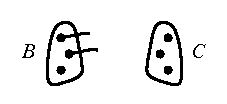
\includegraphics{1437.pdf}                & 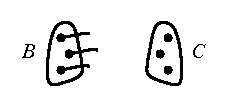
\includegraphics{1438.pdf} \\[-10pt]
   Determinate: $f$ is a function            & Total \\[\lgap]
   
\includegraphics{1437b.pdf}               & 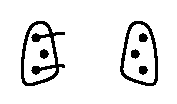
\includegraphics{1438b.pdf} \\[-10pt]
   Not determinate: $\rho$ is not a function & Not total (partial) \\[\llgap] \hline
   One-to-one (14.41b)                       & Onto (14.41a) \\
   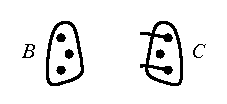
\includegraphics{1441a.pdf}               & 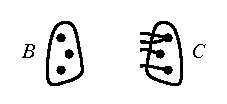
\includegraphics{1441b.pdf} \\[-10pt]
   One-to-one                                & Onto \\[\lgap]
   
\includegraphics{1441ab.pdf}              & 
\includegraphics{1441bb.pdf} \\[-10pt]
   Not one-to-one                            & Not onto \\[\llgap] \hline
\end{tabular}
\end{table}

%\newpage

\subsection*{Order relations}
\begin{tabbing}
(99.99.9)\;\=(m)\;\=\kill
(14.47)\>\textbf{Definition:}\quad A binary relation $\rho$ on a set $B$ is called a \emph{partial order on} $b$ if it is\\[\lgap]
       \>reflexive, antisymmetric, and transitive. In this case, pair $\langle B, \rho\rangle$ is called a \emph{partially}\\[\lgap]
       \>\emph{ordered set} or \emph{poset}.\\[\lgap]
We use the symbol $\preceq$ for an arbitrary partial order, sometimes writing $c\succeq b$ instead of $b\preceq c$.\\[\llgap]
(14.47.1)\>\textbf{Definition, Incomparable:}\quad $incomp(b,c) \equivs \neg (b\preceq c) \land \neg (c\preceq b)$\\[\lgap]
(14.48)\>\textbf{Definition:}\quad Relation $\prec$ is a \emph{quasi order} or \emph{strict partial order} if $\prec$ is trasitive\\[\lgap]
       \>and irreflexive\\[\lgap]
(14.48.1)\>\textbf{Definition, Reflexive reduction:}\quad Given $\preceq$, its \emph{reflexive reduction} $\prec$ is computed\\[\lgap]
         \>by eliminating all pairs $\langle b,b\rangle$ from $\preceq$.\\[\lgap]
(14.48.2)\>Let $\prec$ be the reflexive reduction of $\preceq$. Then,\\[\lgap]
         \>$\neg (b\preceq c) \equivs c\prec b \lor incomp(b,c)$\\[\lgap]
(14.49)\>(a)\>If $\rho$ is a partial order over a set $B$, then $\rho - i_{B}$ is a quasi order.\\[\lgap]
       \>(b)\>If $\rho$ is a quasi order over a set $B$, then $\rho \cup i_{B}$ is a partial order.\\[\lgap]
\end{tabbing}

\subsection*{Total orders and topological sort}
\begin{tabbing}
(99.99.9)\;\=(m)\;\=\kill
(14.50)\>\textbf{Definition:}\quad A partial order $\preceq$ over $B$ is called a \emph{total} or \emph{linear} order if\\[\lgap]
       \>$(\all b,c\drrb b\preceq c \lor b\succeq c)$, i.e. iff $\preceq\cup\preceq^{-1} = B\times B$.\\[\lgap]
       \> In this case, the pair $\langle B,\preceq\rangle$ is called a \emph{linearly ordered set} or a \emph{chain}.\\[\llgap]
(14.51)\>\textbf{Definitions:}\quad Let $S$ be a nonempty subset of poset $\langle U,\preceq\rangle$.\\[\lgap]
       \>(a)\>Element $b$ of $S$ is a \emph{minimal element of} $S$ if no element of $S$ is smaller than $b$,\\[\lgap]
       \>   \>i.e. if $b\in S\land (\all c\dr c \prec b\rb c\notin S)$.\\[\lgap]
       \>(b)\>Element $b$ of $S$ is the \emph{least element of} $S$ if $b\in S\land (\all c\dr c\in S\rb b\preceq c)$.\\[\lgap]
       \>(c)\>Element $b$ is a \emph{lower bound of} $S$ if $(\all c\dr c\in S\rb b\preceq c)$.\\[\lgap]
       \>   \>(A lower bound of $S$ need not be in $S$.)\\[\lgap]
       \>(d)\>Element $b$ is the \emph{greatest lower bound of} $S$, written $glb.S$ if $b$ is a lower bound\\[\lgap]
       \>   \>and if every lower bound $c$ satisfies $c\preceq b$.\\[\llgap]
(14.52)\>Every finite nonempty subset $S$ of poset $\langle U, \preceq\rangle$ has a minimal element.\\[\llgap]
(14.53)\>Let $B$ be a nonempty subset of poset $\langle U, \preceq\rangle$.\\[\lgap]
       \>(a)\>A least element of $B$ is also a minimal element of $B$ (but not necessarily\\[\lgap]
       \>   \>vice versa).\\[\lgap]
       \>(b)\>A least element of $B$ is also a greatest lower bound of $B$ (but not necessarily\\[\lgap]
       \>   \>vice versa).\\[\lgap]
       \>(c)\>A lower bound of $B$ that belongs to $B$ is also a least element of $B$.\\[\llgap]
(14.54)\>\textbf{Definitions:}\quad Let $S$ be a nonempty subset of poset $\langle U, \preceq\rangle$.\\[\lgap]
       \>(a)\>Element $b$ of $S$ is a \emph{maximal element of} $S$ if no element of $S$ is larger than $b$,\\[\lgap]
       \>   \>i.e. if $b \in S\land (\all c\dr b\prec c\rb c\notin S)$.\\[\lgap]
       \>(b)\>Element $b$ of $S$ is the \emph{greatest element of} $S$ if $b\in S\land (\all c\dr c\in S\rb c\preceq b)$.\\[\lgap]
       \>(c)\>Element $b$ is an \emph{upper bound of} $S$ if $(\all c\dr c\in S\rb c\preceq b)$.\\[\lgap]
       \>   \>(An upper bound of $S$ need not be in $S$.)\\[\lgap]
       \>(d)\>Element $b$ is the \emph{least upper bound of} $S$, written $lub.S$, if $b$ is an upper bound\\[\lgap]
       \>   \>and if every upper bound $c$ satisfies $b\preceq c$.\\[\lgap]
\end{tabbing}

\subsection*{Relational databases}
\begin{tabbing}
(99.99.9)\;\=\kill
(14.56.1)\>\textbf{Definition, select:}\quad For Relation $R$ and predicate $F$, which may contain names\\[\lgap]
       \>of fields of $R$, \quad $\sigma (R,F) = \{ t\dr t \in R \land F \}$\\[\llgap]
(14.56.2)\>\textbf{Definition, project:}\quad For $A_{1}, \ldots, A_{m}$ a subset of the names of the fields of\\[\lgap]
       \>relation $R$, \quad $\pi (R,A_{1}, \ldots, A_{m}) = \{ t \dr t\in R \rb \langle t.A_{1}, t.A_{2}, \ldots, t.A_{m}\rangle\}$\\[\llgap]
(14.56.3)\>\textbf{Definition, natural join:}\quad For Relations $R1$ and $R2$, $R1 \bowtie R2$ has all the attributes\\[\lgap]
       \>that $R1$ and $R2$ have, but if an attribute appears in both, then it appears only once in\\[\lgap]
       \>the result; further, only those tuples that agree on this common attribute are included.\\[\llgap]
\end{tabbing}

\section*{A Theory of Integers}
Let $D$ be a set of elements, two of which are 0 and 1, and let $+$ and $\cdot$ be binary operators on $D$.
Assume $D$ is \emph{closed} with respect to $+$ and $\cdot$, i.e. for any $a$ and $b$ in $D$, $a+b$ and
$a \cdot b$ are also in $D$. $D$ is called an \emph{integral domain} if it satisfies axioms (15.1)--(15.7).

\subsection*{Integral domains}
\begin{tabbing}
(99.99.9)\;\=(m)\;\= \makebox[2in]{ } \= \kill
(15.1)\>\textbf{Axiom, Associativity:}\\[\lgap]
      \>   $(a + b) + c = a + (b + c)$
      \>\> $(a \cdot b) \cdot c = a \cdot (b \cdot c)$\\[\lgap]
(15.2)\>\textbf{Axiom, Symmetry:}\\[\lgap]
      \>   $a + b = b + a$
      \>\> $a \cdot b = b \cdot a$\\[\lgap]
(15.3)\>\textbf{Axiom, Additive identity:}\\[\lgap]
      \>   $0 + a = a$
      \>\> $a + 0 = a$\\[\lgap]
(15.4)\>\textbf{Axiom, Multiplicative identity:}\\[\lgap]
      \>   $1 \cdot a = a$
      \>\> $a \cdot 1 = a$\\[\lgap]
(15.5)\>\textbf{Axiom, Distributivity:}\\[\lgap]
      \>   $a \cdot (b + c) = a \cdot b + a \cdot c$
      \>\> $(b + c) \cdot a = b \cdot a + c \cdot a$\\[\lgap]
(15.6)\>\textbf{Axiom, Additive inverse:}\\[\lgap]
      \>   $(\ext x$: $D \drrb x + a = 0)$
      \>\> $(\ext x$: $D \drrb a + x = 0)$\\[\lgap]
(15.7)\>\textbf{Axiom, Cancellation:}\\[\lgap]
      \>   $c \ne 0 \impl (c \cdot a = c \cdot b \equivss a = b)$
      \>\> $c \ne 0 \impl (a \cdot c = b \cdot c \equivss a = b)$\\[\lgap]
(15.8)\>\textbf{Cancellation:}\quad $a + b = a + c \equivss b = c$\\[\lgap]
(15.9)\>\textbf{Zero:}\quad $a \cdot 0 = 0$\\[\lgap]
(15.10)\>\textbf{Unique identity:}\\[\lgap]
      \>   $a + z = a \equivss z = 0$
      \>\> $a \ne 0 \impl (a \cdot z = a \equivss z = 1)$\\[\lgap]
(15.11)\>  $a \cdot b = 0 \equivss a = 0 \lor b = 0$\\[\lgap]
\end{tabbing}

\subsection*{Subtraction}
\begin{tabbing}
(99.99.9)\;\=(m)\;\= \makebox[2in]{ } \= \kill
(15.12)\>\textbf{Unique additive inverse:}\quad $x + a = 0 \land y + a = 0 \;\impl\; x = y$\\[\lgap]
(15.13)\>\textbf{Axiom, Unary minus:}\quad $a + (-a) = 0$\\[\lgap]
(15.14)\>\textbf{Axiom, Subtraction:}\quad $a - b = a + (-b)$\\[\lgap]
(15.15)\>$x + a = 0 \equivss x = -a$\\[\lgap]
(15.16)\>$-a = -b \equivss a = b$\\[\lgap]
(15.17)\>$-(-a) = a$\\[\lgap]
(15.18)\>$-0 = 0$\\[\lgap]
(15.19)\>$-(a + b) = (-a) + (-b)$\\[\lgap]
(15.20)\>$-a = (-1) \cdot a$\\[\lgap]
(15.21)\>$(-a) \cdot b = a \cdot (-b)$\\[\lgap]
(15.22)\>$a \cdot (-b) = -(a \cdot b)$\\[\lgap]
(15.23)\>$(-a) \cdot (-b) = a \cdot b$\\[\lgap]
(15.24)\>$a - 0 = a$\\[\lgap]
(15.25)\>$(a - b) + (c - d) = (a + c) - (b + d)$\\[\lgap]
(15.26)\>$(a - b) - (c - d) = (a + d) - (b + c)$\\[\lgap]
(15.27)\>$(a - b) \cdot (c - d) = (a \cdot c + b \cdot d) - (a \cdot d + b \cdot c)$\\[\lgap]
(15.28)\>$a - b = c - d \equivss a + d = b + c$\\[\lgap]
(15.29)\>$(a - b) \cdot c = a \cdot c - b \cdot c$\\[\lgap]
\end{tabbing}

\subsection*{Ordered domains}
An integral domain $D$ with predicate $pos$ that satisfies axioms (15.30)--(15.33) is called an
\emph{ordered domain}, and the ordering is a \emph{total} or \emph{linear} order as defined in (14.50).
\begin{tabbing}
(99.99.9)\;\=(m)\;\= \makebox[2in]{ } \= \kill
(15.30)\>\textbf{Axiom, Addition:}\quad $pos.a \land pos.b \impl pos(a + b)$\\[\lgap]
(15.31)\>\textbf{Axiom, Multiplication:}\quad $pos.a \land pos.b \impl pos(a \cdot b)$\\[\lgap]
(15.32)\>\textbf{Axiom:}\quad $\neg pos.0$\\[\lgap]
(15.33)\>\textbf{Axiom:}\quad $b \ne 0 \;\impl\; (pos.b \equiv \neg pos(-b))$\\[\llgap]
(15.34)\>$b \ne 0 \impl pos(b \cdot b)$\\[\lgap]
(15.35)\>$pos.a \impl (pos.b \equiv pos(a \cdot b))$\\[\llgap]
(15.36)\>\textbf{Axiom, Less:}\quad $a < b \equivs pos(b - a)$\\[\lgap]
(15.37)\>\textbf{Axiom, Greater:}\quad $a > b \equivs pos(a - b)$\\[\lgap]
(15.38)\>\textbf{Axiom, At most:}\quad $a \le b \equivs a < b \lor a = b$\\[\lgap]
(15.39)\>\textbf{Axiom, At least:}\quad $a \ge b \equivs a > b \lor a = b$\\[\llgap]
(15.40)\>\textbf{Positive elements:}\quad $pos.b \equivs 0 < b$\\[\lgap]
(15.41)\>\textbf{Transitivity:}\\[\lgap]
       \>(a)\> $a < b \land b < c \impl a < c$\\[\lgap]
       \>(b)\> $a \le b \land b < c \impl a < c$\\[\lgap]
       \>(c)\> $a < b \land b \le c \impl a < c$\\[\lgap]
       \>(d)\> $a \le b \land b \le c \impl a \le c$\\[\lgap]
(15.42)\>\textbf{Monotonicity:}\quad $a < b \equivss a + d < b + d$\\[\lgap]
(15.43)\>\textbf{Monotonicity:}\quad $0 < d \;\impl\; (a < b \equiv a \cdot d < b \cdot d)$\\[\lgap]
(15.44)\>\textbf{Tricotomy:}\quad $(a < b \equivss a = b \equivss a > b) \;\land\; \neg (a < b \;\land\; a = b \;\land\; a > b)$\\[\lgap]
(15.45)\>\textbf{Antisymmetry:}\quad $a \le b \land b \le a \equivss a = b$\\[\lgap]
(15.46)\>\textbf{Reflexivity:}\quad $a \le a$\\[\lgap]
(15.47)\>$a = b \equivss (\all z$: $D \drrb z \le a \equivs z \le b)$\\[\lgap]
\end{tabbing}

\subsection*{Well-ordered domains}
A subset $D'$ of an ordered domain is called \emph{well ordered} if each nonempty subset $S$ of $D'$
contains a minimal element (according to relation $<$):
\begin{tabbing}
(99.99.9)\;\=(m)\;\= \makebox[2in]{ } \= \kill
(15.48)\>$S \ne 0 \equivs (\ext b\dr b \in S \rb (\all c \dr c < b \rb c \notin S))$\quad for all $S \subseteq D'$\\[\lgap]
(15.49)\>\textbf{Axiom, Well ordering:}\quad The set $\mathbb{N}$ of natural numbers is well ordered\\[\lgap]
       \>(under the ordering $<$ defined in (15.36)).\\[\lgap]
(15.50)\>In a well-ordered domain, there is no element between 0 and 1.\\[\lgap]
\end{tabbing}

\subsection*{Quantification for $\;+\;$ and $\;\cdot\;$}
\begin{tabbing}
(99.99.9)\;\=(m)\;\= \makebox[2in]{ } \= \kill
(15.51)\>\textbf{Axiom, Distributivity:}\quad $Q \cdot (\Sigma x \dr R \rb P) = (\Sigma x \dr R \rb Q \cdot P)$\\[\lgap]
\end{tabbing}

\subsection*{Minimum and maximum}
\begin{tabbing}
(99.99.9)\;\=(m)\;\= \makebox[2in]{ } \= \kill
(15.53)\>\textbf{Definition of $\downarrow$ :}\quad $(\all z\drrb z\le \;x\downarrow y\equivs z\le x \land z\le y)$\\[\lgap]
       \>\textbf{Definition of $\uparrow$ :}\quad $(\all z\drrb z\ge \;x\uparrow y\equivs z\ge x \land z\ge y)$\\[\lgap]
(15.54)\>\textbf{Symmetry:}\\[\lgap]
       \>$x\downarrow y \;=\; y\downarrow x$ \>\> $x\uparrow y \;=\; y\uparrow x$\\[\lgap]
(15.55)\>\textbf{Associativity:}\\[\lgap]
       \>$(x\downarrow y)\downarrow z \;=\; x\downarrow (y\downarrow z)$ \>\> $(x\uparrow y)\uparrow z \;=\; x\uparrow (y\uparrow z)$\\[\lgap]
\end{tabbing}

\subsection*{Restrictions.}
Although $\downarrow$ and $\uparrow$ are symmetric and associative, they do not have identities over the integers.
Therefore, axiom (8.13) empty range does not apply to $\downarrow$ or $\uparrow$. Also, when using range-split
axioms, no range should be \emph{false}.\\[\lgap]

\begin{tabbing}
(99.99.9)\;\=(m)\;\= \makebox[2in]{ } \= \kill
(15.56)\>\textbf{Idempotency:}\\[\lgap]
       \>$x\downarrow x \;=\; x$ \>\> $x\uparrow x \;=\; x$\\[\lgap]
(15.57)\>$x\downarrow y\;\le x \;\land\; x\downarrow y\;\le y$ \>\> $x\uparrow y\;\ge x \;\land\; x\uparrow y\;\ge y$\\[\lgap]
(15.58)\>$x\le y \equivs x\downarrow y \;= x$ \>\> $x\ge y \equivs x\uparrow y \;= x$\\[\lgap]
(15.59)\>$x\downarrow y\; = x \;\lor\; x\downarrow y = y$ \>\> $x\uparrow y\; = x \;\lor\; x\uparrow y = y$\\[\lgap]
(15.60)\>\textbf{Distributivity:}\\[\lgap]
       \>$c + (x\downarrow y) \;=\; (c + x)\downarrow (c + y)$ \>\> $c + (x\uparrow y) \;=\; (c + x)\uparrow (c + y)$\\[\lgap]
(15.61)\>\textbf{Distributivity:}\\[\lgap]
       \>$c\ge 0\impls c\cdot (x\downarrow y) \;=\; (c\cdot x)\downarrow (c\cdot y)$\\[\lgap]
       \>$c\ge 0\impls c\cdot (x\uparrow y) \;=\; (c\cdot x)\uparrow (c\cdot y)$\\[\lgap]
(15.62)\>\textbf{Distributivity:}\\[\lgap]
       \>$c\le 0\impls c\cdot (x\uparrow y) \;=\; (c\cdot x)\downarrow (c\cdot y)$\\[\lgap]
       \>$c\le 0\impls c\cdot (x\downarrow y) \;=\; (c\cdot x)\uparrow (c\cdot y)$\\[\llgap]
(15.64)\>\textbf{Distributivity of $+$ over $\downarrow$ :}\quad Provided $\neg occurs(\Lq x\Rq ,\Lq E\Rq)$,\\[\lgap]
       \>$(\ext x\drrb R) \impls E + (\downarrow x\dr R\rb P) = (\downarrow x\dr R\rb E + P)$\\[\lgap]
(15.65)\>\textbf{Distributivity of $+$ over $\uparrow$ :}\quad Provided $\neg occurs(\Lq x\Rq ,\Lq E\Rq)$,\\[\lgap]
       \>$(\ext x\drrb R) \impls E + (\uparrow x\dr R\rb P) = (\uparrow x\dr R\rb E + P)$\\[\lgap]
(15.66)\>\textbf{Distributivity of $\cdot$ over $\downarrow$ :}\quad Provided $\neg occurs(\Lq x\Rq ,\Lq E\Rq)$,\\[\lgap]
       \>$(\ext x\drrb R) \land E\ge 0 \impls E\cdot (\downarrow x\dr R\rb P) = (\downarrow x\dr R\rb E\cdot P)$\\[\lgap]
(15.67)\>\textbf{Distributivity of $\cdot$ over $\uparrow$ :}\quad Provided $\neg occurs(\Lq x\Rq ,\Lq E\Rq)$,\\[\lgap]
       \>$(\ext x\drrb R) \land E\ge 0 \impls E\cdot (\uparrow x\dr R\rb P) = (\uparrow x\dr R\rb E\cdot P)$\\[\lgap]
(15.68)\>\textbf{Distributivity of $\downarrow$ over $\uparrow$ :}\quad Provided $\neg occurs(\Lq x\Rq ,\Lq E\Rq)$,\\[\lgap]
       \>$E\downarrow (\uparrow x\dr R\rb P) = (\uparrow x\dr R\rb E\downarrow P)$\\[\lgap]
(15.69)\>\textbf{Distributivity of $\uparrow$ over $\downarrow$ :}\quad Provided $\neg occurs(\Lq x\Rq ,\Lq E\Rq)$,\\[\lgap]
       \>$E\uparrow (\downarrow x\dr R\rb P) = (\downarrow x\dr R\rb E\uparrow P)$\\[\lgap]
\end{tabbing}

\newpage

\begin{tabbing}
(99.99.9)\;\=(m)\;\= \makebox[2in]{ } \= \kill
(15.70)\>Provided $\neg occurs(\Lq x\Rq ,\Lq E\Rq)$,\\[\lgap]
       \>$R[x := E] \impls E=E \uparrow (\downarrow x\dr R\rb x)$\\[\lgap]
       \>$R[x := E] \impls E=E \downarrow (\uparrow x\dr R\rb x)$\\[\lgap]
\end{tabbing}

\subsection*{Absolute value}
\begin{tabbing}
(99.99.9)\;\=(m)\;\= \makebox[2in]{ } \= \kill
(15.71)\>\textbf{Definition of $abs$ :}\quad $abs.x = x\uparrow -x$\\[\lgap]
(15.72)\>$abs.x = abs(-x)$\\[\lgap]
(15.73)\>\textbf{Triangle inequality:}\quad $abs(x+y) \le abs.x + abs.y$\\[\lgap]
(15.74)\>$abs(abs.x) = abs.x$\\[\lgap]
(15.75)\>$abs(x\cdot y) = abs.x\cdot abs.y$\\[\lgap]
(15.76)\>$-(abs.x + abs.y) \le x + y \le abs.x + abs.y$\\[\lgap]
\end{tabbing}

\subsection*{Divisibility}
\begin{tabbing}
(99.99.9)\;\=(m)\;\= \kill
(15.77)\>\textbf{Definition of $\mid$ :}\quad $c \mid b \equivs (\ext d\drrb c\cdot d = b)$\\[\lgap]
(15.78)\>$c \mid c$\\[\lgap]
(15.79)\>$c \mid 0$\\[\lgap]
(15.80)\>$1 \mid b$\\[\lgap]
(15.80.1)\>$-b \mid c \equivs b \mid c$\\[\lgap]
(15.81)\>$c \mid 1 \impls c=1 \lor c=-1$\\[\lgap]
(15.81.1)\>$c \mid 1 \equivs c=1 \lor c=-1$\\[\lgap]
(15.82)\>$d \mid c \land c \mid b \impls d \mid b$\\[\lgap]
(15.83)\>$b \mid c \land c \mid b \equivss b=c \lor b=-c$\\[\lgap]
(15.84)\>$b \mid c \impls b \mid c\cdot d$\\[\lgap]
(15.85)\>$b \mid c \impls b\cdot d \mid c\cdot d$\\[\lgap]
(15.86)\>$1<b \land b \mid c \impls \neg(b \mid (c+1))$\\[\lgap]
\end{tabbing}

\begin{tabbing}
(99.99.9)\;\=(m)\;\= \makebox[2in]{ } \= \kill
(15.87)\>\textbf{Theorem:}\quad Given integers $b$, $c$ with $c > 0$, there exist (unique) integers $q$ and $r$\\[\lgap]
       \>such that $b=q\cdot c + r$, where $0\le r < c$.\\[\lgap]
(15.89)\>\textbf{Corollary:}\quad For given $b$, $c$, the values $q$ and $r$ of Theorem (15.87) are unique.\\[\lgap]
\end{tabbing}

\subsection*{Greatest common divisor}
\begin{tabbing}
(99.99.9)\;\=(m)\;\= \makebox[2in]{ } \= \kill
(15.90)\>\textbf{Definition of $\div$ and mod for operands $b$ and $c$, $c\ne 0$ :}\\[\lgap]
       \> $b \div c = q, \; b \mymod c = r$ \quad where $b = q\cdot c + r$ and $0 \le r < c$\\[\lgap]
(15.91)\>$b = c\cdot (b \div c) + b \mymod c$\quad for $c\ne 0$\\[\llgap]
(15.92)\>\textbf{Definition of gcd:}\\[\lgap]
       \> $b \mygcd c = (\uparrow d\dr d \mid b \land d \mid c \rb d)$\quad for $b$, $c$ not both 0\\[\lgap]
       \> $0 \mygcd 0 = 0$\\[\lgap]
(15.94)\>\textbf{Definition of lcm :}\\[\lgap]
       \> $b \mylcm c = (\downarrow k$: $\mathbb{Z}^{+}\dr b\mid k \land c \mid k \rb k)$\quad for $b\ne 0$ and $c\ne 0$\\[\lgap]
       \> $b \mylcm c = 0$\quad for $b=0$ or $c=0$\\[\lgap]
\end{tabbing}

\subsection*{Properties of gcd}
\begin{tabbing}
(99.99.9)\;\=(m)\;\= \makebox[2in]{ } \= \kill
(15.96)\>\textbf{Symmetry:}\quad $b \mygcd c = c \mygcd b$\\[\lgap]
(15.97)\>\textbf{Associativity:}\quad $(b \mygcd c) \mygcd d = b \mygcd (c \mygcd d)$\\[\lgap]
(15.98)\>\textbf{Idempotency:}\quad $(b \mygcd b) = abs.b$\\[\lgap]
(15.99)\>\textbf{Zero:}\quad $1 \mygcd b = 1$\\[\lgap]
(15.100)\>\textbf{Identity:}\quad $0 \mygcd b = abs.b$\\[\lgap]
(15.101)\>$b \mygcd c = (abs.b) \mygcd (abs.c)$\\[\lgap]
(15.102)\>$b \mygcd c = b \mygcd (b + c) = b \mygcd (b - c)$\\[\lgap]
(15.103)\>$b = a\cdot c + d \impls b \mygcd c = c \mygcd d$\\[\lgap]
(15.104)\>\textbf{Distributivity:}\quad $d \cdot (b \mygcd c) = (d \cdot b) \mygcd (d\cdot c)$\\[\llgap]
(15.105)\>\textbf{Definition of relatively prime $\perp$ :}\quad $b \perp c \equivs b \mygcd c = 1$\\[\llgap]
(15.107)\>\textbf{Inductive definition of gcd:}\\[\lgap]
       \> $b \mygcd 0 = b$\\[\lgap]
       \> $b \mygcd c = c \mygcd (b \mymod c)$\\[\llgap]
(15.108)\>$(\ext x, y\drrb x\cdot b + y\cdot c = b \mygcd c$\quad for all $b,c$: $\mathbb{N}$\\[\lgap]
(15.111)\>$k \mid b \;\land\; k \mid c \equivss k \mid (b \mygcd c)$\\[\lgap]
\end{tabbing}

\section*{Growth of Functions}
\begin{tabbing}
(99.99.9)\;\=(m)\;\= \makebox[2in]{ } \= \kill
(g.1)\>\textbf{Definition of asymptotic upper bound:}\quad For a given function $g.n$, \;$O(g.n)$,\\[\lgap]
     \> pronounced ``big-oh of $g$ of $n$'', is the set of functions\\[\lgap]
     \> $\{f.n \dr (\ext c,n_{0}\dr c>0 \land n_{0}>0 \rb (\all n \dr n\ge n_{0} \rb 0\le f.n\le c \cdot g.n)\;)\}$\\[\lgap]
(g.2)\>\textbf{$O$-notation:}\quad $f.n = O(g.n)$ means function $f.n$ is in the set $O(g.n).$\\[\llgap]
(g.3)\>\textbf{Definition of asymptotic lower bound:}\quad For a given function $g.n$, \;$\Omega(g.n)$,\\[\lgap]
     \> pronounced ``big-omega of $g$ of $n$'', is the set of functions\\[\lgap]
     \> $\{f.n \dr (\ext c,n_{0}\dr c>0 \land n_{0}>0 \rb (\all n \dr n\ge n_{0} \rb 0\le c \cdot g.n\le f.n)\;)\}$\\[\lgap]
(g.4)\>\textbf{$\Omega$-notation:}\quad $f.n = \Omega(g.n)$ means function $f.n$ is in the set $\Omega(g.n).$\\[\llgap]
(g.5)\>\textbf{Definition:}\quad $f.n = \Theta (g.n)$ if and only if $f.n = O(g.n)$ and $f.n = \Omega (g.n)$\\[\lgap]
(g.6)\>$\Theta (g.n)$ is the set of functions $\{f.n \dr (\ext c_{1},c_{2},n_{0}\dr c_{1}>0 \land c_{2}>0 \land n_{0}>0 \rb$\\[\lgap]
     \>$(\all n \dr n\ge n_{0} \rb 0 \;\le\; c_{1} \cdot g.n \;\le\; f.n \;\le\; c_{2} \cdot g.n)\;)\}$\\[\lgap]
     \end{tabbing}

\subsection*{Comparison of functions}
\begin{tabbing}
(99.99.9)\;\=(m)\;\= \makebox[2in]{ } \= \kill
(g.7)\>\textbf{Reflexivity:}\\[\lgap]
     \>(a)\>$f.n = O(f.n)$\\[\lgap]
     \>(b)\>$f.n = \Omega (f.n)$\\[\lgap]
     \>(c)\>$f.n = \Theta (f.n)$\\[\lgap]
(g.8)\>\textbf{Symmetry:}\quad $f.n = \Theta (g.n) \equivs g.n = \Theta (f.n)$\\[\lgap]
(g.9)\>\textbf{Transpose symmetry:}\quad $f.n = O(g.n) \equivs g.n = \Omega (f.n)$\\[\lgap]
\end{tabbing}

\newpage

\begin{tabbing}
(99.99.9)\;\=(m)\;\= \makebox[2in]{ } \= \kill
(g.10)\>\textbf{Transitivity:}\\[\lgap]
     \>(a)\>$f.n = O(g.n) \;\land\; g.n = O(h.n) \;\impl\; f.n = O(h.n)$\\[\lgap]
     \>(b)\>$f.n = \Omega (g.n) \;\land\; g.n = \Omega (h.n) \;\impl\; f.n = \Omega (h.n)$\\[\lgap]
     \>(b)\>$f.n = \Theta (g.n) \;\land\; g.n = \Theta (h.n) \;\impl\; f.n = \Theta (h.n)$\\[\llgap]
(g.11)\>Define an \emph{asymptotically positive polynomial $p.n$ of degree $d$} to be\\[\lgap]
      \>$p(n) = (\Sigma i\dr 0\le i\le d \rb a_{i}n^{i})$ where the constants $a_{0}, a_{1}, \ldots , a_{d}$ are the\\[\lgap]
      \>\emph{coefficients} of the polynomial and $a_{d} > 0$. Then $p.n = \Theta(n^{d})$.\\[\llgap]
(g.12)\>(a)\>$O (1) \subset O (\lg n) \subset O (n) \subset O (n\lg n) \subset O (n^{2}) \subset O (n^{3}) \subset O (2^{n})$\\[\lgap]
      \>(b)\>$\Omega (1) \supset \Omega (\lg n) \supset \Omega (n) \supset \Omega (n\lg n) \supset \Omega (n^{2}) \supset \Omega (n^{3}) \supset \Omega (2^{n})$\\[\lgap]
\end{tabbing}

\section*{Combinatorial Analysis}
\begin{tabbing}
(99.99.9)\;\=(m)\;\= \makebox[2in]{ } \= \kill
(16.1)\>\textbf{Rule of sum:}\quad The size of the union of $n$ (finite) pairwise disjoint sets is the\\[\lgap]
      \>sum of their sizes.\\[\llgap]
(16.2)\>\textbf{Rule of product:}\quad The size of the cross product of $n$ sets is the product of\\[\lgap]
      \>their sizes.\\[\llgap]
(16.3)\>\textbf{Rule of difference:}\quad The size of a set with a subset of it removed is the size of\\[\lgap]
      \>the set minus the size of the subset.\\[\llgap]
(16.4)\>\textbf{Definition:}\quad $P(n,r)=n!/(n-r)!$\\[\lgap]
(16.5)\>The number of $r$-permutations of a set of size $n$ equals $P(n,r)$.\\[\lgap]
(16.6)\>The number of $r$-permutations with repetition of a set of size $n$ is $n^{r}$.\\[\lgap]
(16.7)\>The number of permutations of a bag of size $n$ with $k$ distinct elements occurring\\[\lgap]
      \>$n_{1},n_{2}, \ldots ,n_{k}$ times is $\dfrac{n!}{n_{1}!\cdot n_{2}!\cdot \cdots \cdot n_{k}!}$.\\[\llgap]
(16.9)\>\textbf{Definition:}\quad The \emph{binomial coefficient} $\binom{n}{r}$, which is read as ``$n$ choose $r$'', is\\[\lgap]
      \>defined by \quad $\dbinom{n}{r} = \dfrac{n!}{r!\cdot (n-r)!}$ \quad for $0\le r \le n$.\\[\llgap]
(16.10)\>The number of $r$-combinations of $n$ elements is $\binom{n}{r}$.\\[\llgap]
(16.11)\>The number $\binom{n}{r}$ of $r$-combinations of a set of size $n$ equals the number of\\[\lgap]
       \>permutations of a bag that contains $r$ copies of one object and $n-r$ copies of\\[\lgap]
       \>another.\\[\lgap]
\end{tabbing}

\section*{A Theory of Graphs}
\begin{tabbing}
(99.99.9)\;\=(m)\;\= \makebox[2in]{ } \= \kill
(19.1)\>\textbf{Definition:}\quad Let $V$ be a finite, nonempty set and $E$ a binary relation on $V$.\\[\lgap]
      \>Then $G=\langle V,E\rangle$ is called a \emph{directed graph}, or \emph{digraph}. An element of $V$ is\\[\lgap]
      \>called a \emph{vertex}; an element of $E$ is called an \emph{edge}.\\[\llgap]
(19.1.1)\>\textbf{Definitions:}\\[\lgap]
      \>(a)\>In an \emph{undirected} graph $\langle V,E\rangle$, $E$ is a set of \emph{unordered} pairs.\\[\lgap]
      \>(b)\>In a \emph{multigraph} $\langle V,E\rangle$, $E$ is a \emph{bag} of undirected edges.\\[\lgap]
      \>(c)\>The \emph{indegree} of a vertex of a digraph is the number of edges for which it is\\[\lgap]
      \>   \>an end vertex.\\[\lgap]
      \>(d)\>The \emph{outdegree} of a vertex of a digraph is the number of edges for which it is\\[\lgap]
      \>   \>a start vertex.\\[\lgap]
      \>(e)\>The \emph{degree} of a vertex is the sum of its indegree and outdegree.\\[\lgap]
      \>(f)\>An edge $\langle b,b\rangle$ for some vertex $b$ is a \emph{self-loop}.\\[\lgap]
      \>(g)\>A digraph with no self-loops is called \emph{loop-free}.\\[\llgap]
(19.3)\>The sum of the degrees of the vertices of a digraph or multigraph equals $2\cdot\# E$.\\[\lgap]
(19.4)\>In a digraph or multigraph, the number of vertices of odd degree is even.\\[\llgap]
(19.4.1)\>\textbf{Definition:}\quad A \emph{path} has the following properties.\\[\lgap]
      \>(a)\>A path starts with a vertex, ends with a vertex, and alternates between\\[\lgap]
      \>   \>vertices and edges.\\[\lgap]
      \>(b)\>Each directed edge in a path is preceded by its start vertex and followed by\\[\lgap]
      \>   \>its end vertex. An undirected edge is preceded by one of its vertices and\\[\lgap]
      \>   \>followed by the other.\\[\lgap]
      \>(c)\>No edge appears more than once.\\[\llgap]
(19.4.2)\>\textbf{Definitions:}\\[\lgap]
      \>(a)\>A \emph{simple} path is a path in which no vertex appears more than once, except\\[\lgap]
      \>   \>that the first and last vertices may be the same.\\[\lgap]
      \>(b)\>A \emph{cycle} is a path with at least one edge, and with the first and last vertices\\[\lgap]
      \>   \>the same.\\[\lgap]
      \>(c)\>An undirected multigraph is \emph{connected} if there is a path between any two\\[\lgap]
      \>   \>vertices.\\[\lgap]
      \>(d)\>A digraph is \emph{connected} if making its edges undirected results in a connected\\[\lgap]
      \>   \>multigraph.\\[\llgap]
(19.6)\>If a graph has a path from vertex $b$ to vertex $c$, then it has a simple path from $b$ to $c$.\\[\llgap]
(19.6.1)\>\textbf{Definitions:}\\[\lgap]
      \>(a)\>An \emph{Euler path} of a multigraph is a path that contains each edge of the graph\\[\lgap]
      \>   \>exactly once.\\[\lgap]
      \>(b)\>An \emph{Euler circuit} is an Euler path whose first and last vertices are the same.\\[\llgap]
(19.8)\>An undirected connected multigraph has an Euler circuit iff every vertex has even\\[\lgap]
      \>degree.\\[\llgap]
(19.8.1)\>\textbf{Definitions:}\\[\lgap]
      \>(a)\>A \emph{complete graph} with $n$ vertices, denoted by $K_{n}$, is an undirected, loop-\\[\lgap]
      \>   \>free graph in which there is an edge between every pair of distinct vertices.\\[\lgap]
      \>(b)\>A \emph{bipartite graph} is an undirected graph in which the set of vertices are\\[\lgap]
      \>   \>partitioned into two sets $X$ and $Y$ such that each edge is incident on one\\[\lgap]
      \>   \>vertex in $X$ and one vertex in $Y$.\\[\llgap]
\end{tabbing}

\newpage

\begin{tabbing}
(99.99.9)\;\=(m)\;\= \makebox[2in]{ } \= \kill
(19.10)\>A path of a bipartate graph is of even length iff its ends are in the same partition\\[\lgap]
       \>element.\\[\lgap]
(19.11)\>A connected graph is bipartate iff every cycle has even length.\\[\llgap]
(19.11.1)\>\textbf{Definition:}\quad A \emph{complete bipartate graph} $K_{m,n}$ is a bipartite graph in which\\[\lgap]
         \>one partition element $X$ has $m$ vertices, the other partition element $Y$ has $n$\\[\lgap]
         \> vertices, and there is an edge between each vertex of $X$ and each vertex of $Y$.\\[\llgap]
(19.11.2)\>\textbf{Definitions:}\\[\lgap]
      \>(a)\>A \emph{Hamilton path} of a graph or digraph is a path that contains each vertex\\[\lgap]
      \>   \>exactly once, except that the end vertices of the path may be the same.\\[\lgap]
      \>(b)\>A \emph{Hamilton circuit} is a Hamilton path that is a cycle.\\[\lgap]
\end{tabbing}

\section*{A Theory of Programs}
\begin{tabbing}
(99.99.9)\;\=(m)\;\= \makebox[2in]{ } \= \kill
(p.1)\>\textbf{Axiom, Excluded miracle:}\quad $wp.S.$ \emph{false} $\equiv$\; \emph{false}\\[\lgap]
(p.2)\>\textbf{Axiom, Conjunctivity:}\quad $wp.S.(X\land Y) \equivs wp.S.X \land wp.S.Y$\\[\lgap]
(p.3)\>\textbf{Monotonicity:}\quad $(X\impl Y) \impls (wp.S.X \impl wp.S.Y)$\\[\lgap]
(p.4)\>\textbf{Definition, Hoare triple:}\quad $\{Q\} \; S \; \{R\} \equivss Q \impl wp.S.R$\\[\lgap]
(p.5)\>\textbf{Postcondition rule:}\quad $\{Q\} \; S \; \{A\}\land (A\impl R)\; \impl \;\{Q\} \; S \; \{R\}$\\[\lgap]
(p.6)\>\textbf{Definition, Program equivalence:}\quad $S=T\equivss ($For all $R, wp.S.R\equiv wp.T.R)$\\[\lgap]
(p.7)\>$(Q\impl A)\land \{A\}\; S\; \{R\}\; \impl \; \{Q\}\; S\; \{R\} $\\[\lgap]
(p.8)\>$\{Q0\}\; S\; \{R0\}\;\land \{Q1\}\; S\; \{R1\}\; \impl \; \{Q0 \land Q1\}\; S\; \{R0\land R1\}$\\[\lgap]
(p.9)\>$\{Q0\}\; S\; \{R0\}\;\land \{Q1\}\; S\; \{R1\}\; \impl \; \{Q0 \lor Q1\}\; S\; \{R0\lor R1\}$\\[\llgap]
(p.10)\>\textbf{Definition, skip:}\quad $wp.$\emph{skip}$.R \equivs R$\\[\lgap]
(p.11)\>$\{Q\}\; $\emph{skip}$\; \{R\} \equivss Q\impl R$\\[\lgap]
(p.12)\>\textbf{Definition, abort:}\quad $wp.$\emph{abort}$.R \equivs $ \emph{false}\\[\lgap]
(p.13)\>$\{Q\}\; $\emph{abort}$\; \{R\} \equivss Q\equiv\;$ \emph{false}\\[\lgap]
(p.14)\>\textbf{Definition, Composition:}\quad $wp.(S;T).R \equivs wp.S.(wp.T.R)$\\[\lgap]
(p.15)\>$\{Q\}\;S\;\{H\}\;\;\land\;\; \{H\}\;T\;\{R\} \;\; \impl\;\; \{Q\}\;S;T\;\{R\}$\\[\lgap]
(p.16)\>\textbf{Identity of composition:}\\[\lgap]
       \>$S\;;\;$\emph{skip}$\;=S$ \>\> \emph{skip}$\;;S\;=S$\\[\lgap]
(p.17)\>\textbf{Zero of composition:}\\[\lgap]
       \>$S\;;\;$\emph{abort}$\;=\;$\emph{abort} \>\> \emph{abort}$\;;S\;=\;$\emph{abort}\\[\lgap]
(p.18)\>\textbf{Definition, Assignment:}\quad $wp.(x:=E).R \equivs R[x:=E]$\\[\lgap]
(p.19)\>\textbf{Proof method for assignment:}\`(p.19) is (10.2)\\[\lgap]
      \>To show that $x := E$ is an implementation of $\{Q\}x:=?\{R\}$,\\[\lgap]
      \>prove $Q\impl R[x:=E]$.\\[\lgap]
(p.20)\>$(x:=x)=\;$\emph{skip}\\[\lgap]
(p.21)\>$IFG:$\`(p.21) is (10.6)\\[\lgap]
      \>\textbf{if} $B1\to S1$\\[\lgap]
      \>\guard\: $B2\to S2$\\[\lgap]
      \>\guard\: $B3\to S3$\\[\lgap]
      \>\textbf{fi}\\[\lgap]
(p.22)\>\textbf{Definition, }$IFG$\textbf{:}\quad $wp.IFG.R\equivss (B1\lor B2\lor B3)\quad \land$\\[\lgap]
      \>$B1\impl wp.S1.R \;\;\land \;\;B2\impl wp.S2.R \;\;\land \;\;B3\impl wp.S3.R$\\[\lgap]
(p.23)\>\textbf{Empty guard:}\quad \textbf{if}\;\;\textbf{fi}\;\;=\;\;\emph{abort}\\[\lgap]
(p.24)\>\textbf{Proof method for IFG:}\`(p.24) is (10.7)\\[\lgap]
      \>$\{Q\}\;IFG\;\{R\}\equivss (Q\impl B1\lor B2\lor B3)\quad \land$\\[\lgap]
      \>$\{Q\land B1\}\;S1\;\{R\}\;\;\land\;\; \{Q\land B2\}\;S2\;\{R\}\;\;\land\;\; \{Q\land B3\}\;S3\;\{R\}$\\[\lgap]
(p.25)\>$\neg(B1\lor B2\lor B3)\impl\; IFG\;=\;$ \emph{abort}\\[\lgap]
(p.26)\>\textbf{One-guard rule:}\quad $\{Q\}\;\textbf{if }B\to S\textbf{ fi}\; \{R\}\;\impl\; \{Q\}\;S\; \{R\}$\\[\lgap]
(p.27)\>\textbf{Distributivity of program over alternation:}\quad \\[\lgap]
      \>$\textbf{if }B1\to S1;T\;$\guard$\; B2\to S2;T\textbf{ fi}\; =\; \textbf{if }B1\to S1\;$\guard$\; B2\to S2\textbf{ fi}\;;T$\\[\lgap]

\end{tabbing}


\end{document}
